%%%%%%%%%%%%%%%%%%%%%%%%%%%%%%%%%%%%%%%%%%%%%%%%%%%%%%%%%%%%%%%%%%%%%%%%%%%%%%%%%%%%%%%

%   8888888b.                                         888      888
%   888   Y88b                                        888      888
%   888    888                                        888      888
%   888   d88P 888d888 .d88b.   8888b.  88888b.d88b.  88888b.  888  .d88b.
%   8888888P"  888P"  d8P  Y8b     "88b 888 "888 "88b 888 "88b 888 d8P  Y8b
%   888        888    88888888 .d888888 888  888  888 888  888 888 88888888
%   888        888    Y8b.     888  888 888  888  888 888 d88P 888 Y8b.
%   888        888     "Y8888  "Y888888 888  888  888 88888P"  888  "Y8888

%%%%%%%%%%%%%%%%%%%%%%%%%%%%%%%%%%%%%%%%%%%%%%%%%%%%%%%%%%%%%%%%%%%%%%%%%%%%%%%%%%%%%%%

% vscode extension LaTex-Workshop uses these magic comments to 
% define which program will be used to build the project or bibliography
% I do need lualatex to use markdown package. Also, when I use lualatex
% in need to include `pdfencoding=auto` in hyperref setup.
% !TEX program = lualatex

% `-shell-scape` argument doesn't work in Windows 10 lualatex
%% !TEX options = -synctex=1 -interaction=nonstopmode -shell-scape "%DOC%"
% !TEX options = -synctex=1 -interaction=nonstopmode "%DOC%"
% !BIB program = biber

\documentclass[11pt,a4paper,dvipsnames,twoside]{article}

% Document geometry
\usepackage[a4paper,left=3cm,right=2.5cm,vmargin=2.5cm]{geometry}
% \usepackage[showframe,a4paper,left=3cm,right=2.5cm,vmargin=2.5cm]{geometry}

% inputenc is ignored when I'm using lualatex as builder
% \usepackage[utf8]{inputenc}

% To produce a spanish automated output, for instance, TOC is called 'Índice' and
% References is called 'Referencias' (in this case I prefer english)
\usepackage[english]{babel}

% Modifier for space between lines (=\baselinestretch*\baselineskip)
% \renewcommand{\baselinestretch}{1.5}
% Modifies the space between notes in footnotes 
% IMPORTANT: just the same than paragraphs (parskip package below)
% \setlength{\footnotesep}{.9\baselineskip}

% It is better to use setspace package
\usepackage{setspace}
\setstretch{1.5}

% Modifies the space over footnote line
\addtolength{\skip\footins}{\baselineskip}

% To convert fonts already installed in the system and using them as main font in the document
% To check the names that fontspec admits use `otfinfo -i </path/to/font/file/even.ttf>`
% otfinfo does admit also ttf files! For instance:
% `otfinfo -i /usr/share/fonts/liberation/LiberationSerif-Regular.ttf`
\usepackage{fontspec}
\setmainfont{Liberation Serif}
\setsansfont{Liberation Sans}
\setmonofont{CourierPrimeCode-Regular} 
% \setmonofont{Liberation Mono}
% A different font for titles
\newfontfamily\headingfont[]{Liberation Sans}

% To allow custom headings
\usepackage[compact]{titlesec}
\titleformat*{\section}{\Large\headingfont\bfseries}
\titleformat*{\subsection}{\large\headingfont\bfseries}
\titleformat*{\subsubsection}{\normalsize\headingfont\bfseries}
% To control spacing for sections, I'm not using it, it just an example
% \titlespacing*{\section}{3em}{0em}{-2em}

% To change title font family
% \usepackage{titling}
% \renewcommand{\maketitlehooka}{\headingfont}

%%%%%%%%%%%%%%%%%%%%%%%%%%%%%%%%%%%%%%%%%%%%%%%%%%%%%%%%%%%%%%%%%%%%%%%%%%%%%%%%%%%%%%%

%   8888888b.                   888
%   888   Y88b                  888
%   888    888                  888
%   888   d88P 8888b.   .d8888b 888  888  8888b.   .d88b.   .d88b.  .d8888b
%   8888888P"     "88b d88P"    888 .88P     "88b d88P"88b d8P  Y8b 88K
%   888       .d888888 888      888888K  .d888888 888  888 88888888 "Y8888b.
%   888       888  888 Y88b.    888 "88b 888  888 Y88b 888 Y8b.          X88
%   888       "Y888888  "Y8888P 888  888 "Y888888  "Y88888  "Y8888   88888P'
%                                                      888
%                                                 Y8b d88P
%                                                  "Y88P" 

%%%%%%%%%%%%%%%%%%%%%%%%%%%%%%%%%%%%%%%%%%%%%%%%%%%%%%%%%%%%%%%%%%%%%%%%%%%%%%%%%%%%%%%

% biblatex package
% 'block=nbpar' produces a new paragraph for every block (printing the URLs in a new line and preventing breaking short URLs)
% page 50 in https://osl.ugr.es/CTAN/macros/latex/contrib/biblatex/doc/biblatex.pdf
\usepackage[block=par,style=ieee,backend=biber]{biblatex}
\addbibresource{Paper.bib}
\setcounter{biburllcpenalty}{7000}
\setcounter{biburlucpenalty}{7000}
\setcounter{biburlnumpenalty}{7000}

% Basic packages (they don't need extra configurations)
\usepackage{% `esvect` will not work without texlive-fontsextra
  amsmath,
  amsfonts,
  amssymb,
  graphicx,
  multirow,
  tabularx,
  mathtools,
  color,
  url
}

% Improve captions in figures
\usepackage[margin=2.5cm]{caption}
\usepackage{subcaption}
% \setlength{\textfloatsep}{1\baselineskip plus 2\baselineskip minus 2\baselineskip}
% \setlength{\intextsep}{1\baselineskip plus 2\baselineskip minus 2\baselineskip}
% \setlength{\textfloatsep}{1\baselineskip}
\setlength{\intextsep}{1\baselineskip}


% Extra colors
\usepackage[x11names,table]{xcolor}

% To cross references and metadata
\usepackage[]{hyperref}
\hypersetup{%
  pdfencoding=auto,
  pdftitle={Degree Final Project},
  pdfauthor={Javier Fernández // jfernandil@alumnos.unex.es},
  pdfsubject={},
  pdfkeywords={Project, Dendrometry, LoRa, Arduino, IoT},
  colorlinks = false,
  linkbordercolor = DarkGoldenrod2,
  urlbordercolor= DarkGoldenrod2,
  %linkcolor = black,
  %urlcolor  = black,
  breaklinks
}

% To make the frame around UEx seal
\usepackage{mdframed}

% To include References and TOC in the TOC
\usepackage[nottoc]{tocbibind}

% To avoid 'underfull box' warning caused because of bibliography line-break
% \usepackage{etoolbox}
% \apptocmd{\thebibliography}{\raggedright}{}{}

% To use \begin{markdown}\end{markdown} environment and be able to type markdown mode
% IMPORTANT: do not use indent inside \begin{markdown}\end{markdown} environment in the code! 
% if you do lualatex is not translating the markdown code.
\usepackage{markdown}

% To get proper skips between paragraphs when you left a blank line in the code! (so I don't need to use `\\` 
% and I'm not getting warnings all the time) 
% IMPORTANT:
% here is an interesting article speaking about paragraphs an indentation, there are two types of paragraphs; 
% - classic: using indentation to distinguish between one and another
% - modern: dispenses with indents and instead distinguish paragraphs using a blank line between them
% Commenting/uncommenting the following package you can choose between two types.
% more info here: https://tex.stackexchange.com/a/196941/83189
% However this package also has options, which can be
% `indent` (to enable indentation)
% `skip=.5\baselineskip` (by default)
% `parfill` (to impose a minimum space at the end of the last line of a paragraph =30pt by default)
% \usepackage[skip=\baselineskip]{parskip}
% Another different option
% https://tex.stackexchange.com/a/371986/83189
\parskip=.75\baselineskip
\parindent=0pt

% To make quotes (I need renewcommand for mkbegdispquote and mkenddispquote to enable quote marks at the
% end and beginning to displayquote environment. More info: https://tex.stackexchange.com/questions/101809/how-to-force-csquotes-to-show-the-quotations-marks-in-block-quotes)
\usepackage[style=english]{csquotes}
% \renewcommand{\mkbegdispquote}[2]{\openautoquote}
% \renewcommand{\mkenddispquote}[2]{\closeautoquote#1#2}
% \renewcommand{\mkcitation}[1]{ #1}

% Switching to quoting package (for block quotes, I still need csquotes for \enquote{})
\usepackage[begintext=``, endtext='']{quoting}
\quotingsetup{vskip=5pt}

% To print units
\usepackage{siunitx}

% Enumerate lists
\usepackage{enumitem}
% To fix spaces between paragraphs, items and top or bottom fo enumerate/itemize environments I need the following
% see page 3 in https://osl.ugr.es/CTAN/macros/latex/contrib/enumitem/enumitem.pdf
\setlist[itemize]{%
  parsep=.75\baselineskip,
  topsep=0pt,
  partopsep=0pt,
  itemsep=0pt
}
\setlist[enumerate]{%
  parsep=.75\baselineskip,
  topsep=0pt,
  partopsep=0pt,
  itemsep=0pt
}

% To backrefs in the footnotes
\usepackage{footnotebackref}

% To improve headers an footers (I'm using to set page number at right)
\usepackage{fancyhdr}
% Plain style that removes headers but keeps page numbers
\fancypagestyle{plain}{%
  \fancyhf{} % Clears all header and footer fields
  \fancyfoot[R]{\thepage}%
  \renewcommand{\headrulewidth}{0pt}%
  \renewcommand{\footrulewidth}{0pt}%
}
% This style is my custom style
\fancypagestyle{myfancy}{%
	\fancyhf{} % Start with clearing everything in the header and footer
	\renewcommand{\headrulewidth}{1pt} % Makes 1pt width the horizontal rule in header by default
	\fancyfoot[R]{\thepage} % Set the right side of the footer to be the page number
	\fancyhead[R]{\rightmark}
	\setlength{\headheight}{14pt}% ...at least 51.60004pt
}
\pagestyle{myfancy} % Enables by default the custom style.

% To change TOC appearance; see 2.1 section in tocloft.pdf for info about 'titles' option
% it does not mention fancyhdr package but it do the work to flushright page numbers for 
% table of contents pages. see: https://tex.stackexchange.com/a/137301/83189
% \usepackage[titles]{tocloft}
\usepackage{tocloft}
\renewcommand{\cftsecfont}{\headingfont\bfseries}
\renewcommand{\cftsecpagefont}{\headingfont\bfseries}
\renewcommand{\cftsubsecfont}{\headingfont}
\renewcommand{\cftsubsecpagefont}{\headingfont}
\renewcommand{\cftsubsubsecfont}{\headingfont}
\renewcommand{\cftsubsubsecpagefont}{\headingfont}
\tocloftpagestyle{empty} % However, I find better this way bc 'titles' option does not 
% produce a compact TOC, it does expand bc probably it uses the same spacing rules in 
% the TOC than in (subsub)(sub)sections titles at the rest of the text.
% -------------------
% Remove the TOC title (it is redundant if you have included a TOC section inside TOC)
\makeatletter
\renewcommand{\@cftmaketoctitle}{}
\makeatother
% But in the case you still want to print the TOC title, this other one modifies TOC title font
% \renewcommand{\cfttoctitlefont}{\Large\headingfont\bfseries}

% To insert json snippets
\usepackage{listings}
\renewcommand{\lstlistingname}{Example}
% \lstset{%
  % aboveskip=1\baselineskip plus 1\baselineskip minus 2\baselineskip,
  % belowskip=1\baselineskip plus 1\baselineskip minus 2\baselineskip
% }
% \lstset{aboveskip=-18pt plus 2pt, belowskip=-18pt plus 2pt}

% \colorlet{punct}{red!60!black}
% \definecolor{background}{HTML}{EEEEEE}
% \definecolor{delim}{RGB}{20,105,176}
% \colorlet{numb}{magenta!60!black}
\definecolor{punct}{HTML}{0064d3}
\colorlet{background}{gray!20}
\definecolor{delim}{HTML}{ff0000}
\definecolor{numb}{HTML}{0f9d58}

\lstdefinelanguage{json}{%
  % aboveskip=\baselineskip,
  % xleftmargin=2em,
  basicstyle=\scriptsize\ttfamily,
  numbers=left,
  numberstyle=\scriptsize,
  stepnumber=1,
  numbersep=8pt,
  showstringspaces=false,
  breaklines=true,
  frame=lines,
  backgroundcolor=\color{background},
  literate=
   *{0}{{{\color{numb}0}}}{1}
    {1}{{{\color{numb}1}}}{1}
    {2}{{{\color{numb}2}}}{1}
    {3}{{{\color{numb}3}}}{1}
    {4}{{{\color{numb}4}}}{1}
    {5}{{{\color{numb}5}}}{1}
    {6}{{{\color{numb}6}}}{1}
    {7}{{{\color{numb}7}}}{1}
    {8}{{{\color{numb}8}}}{1}
    {9}{{{\color{numb}9}}}{1}
    {:}{{{\color{punct}{:}}}}{1}
    {,}{{{\color{punct}{,}}}}{1}
    {"}{{{\color{punct}{"}}}}{1}
    {\{}{{{\color{delim}{\{}}}}{1}
    {\}}{{{\color{delim}{\}}}}}{1}
    {[}{{{\color{delim}{[}}}}{1}
    {]}{{{\color{delim}{]}}}}{1},
}

\newcommand\YAMLcolonstyle{\color{red}\mdseries}
\newcommand\YAMLkeystyle{\color{black}\mdseries}
\newcommand\YAMLvaluestyle{\color{blue}\mdseries}
% here is a macro expanding to the name of the language
% (handy if you decide to change it further down the road)
\lstdefinelanguage{yaml}{%
  keywords={true,false,null,y,n},
  keywordstyle=\color{darkgray}\bfseries,
  basicstyle=\YAMLkeystyle\scriptsize\ttfamily,
  numbers=left,
  numberstyle=\scriptsize,
  numbersep=8pt,
  breaklines=true,
  frame=lines,
  backgroundcolor=\color{background},
  sensitive=false,
  comment=[l]{\#},
  morecomment=[s]{/*}{*/},
  commentstyle=\color{purple}\ttfamily,
  stringstyle=\YAMLvaluestyle\ttfamily,
  moredelim=[l][\color{orange}]{\&},
  moredelim=[l][\color{magenta}]{*},
  moredelim=**[il][\YAMLcolonstyle{:}\YAMLvaluestyle]{:},   % switch to value style at :
  morestring=[b]',
  morestring=[b]",
  literate = {---}{{\ProcessThreeDashes}}3
             {>}{{\textcolor{red}\textgreater}}1     
             {|}{{\textcolor{red}\textbar}}1 
             {\ -\ }{{\mdseries\ -\ }}3,
}

\definecolor{dkgreen}{rgb}{0,0.6,0}
\definecolor{dred}{rgb}{0.545,0,0}
\definecolor{dblue}{rgb}{0,0,0.545}
% \definecolor{lgrey}{rgb}{0.9,0.9,0.9}
% \definecolor{gray}{rgb}{0.4,0.4,0.4}
\definecolor{darkblue}{rgb}{0.0,0.0,0.6}
\lstdefinelanguage{cpp}{
      backgroundcolor=\color{background},  
      basicstyle=\color{black}\mdseries\scriptsize\ttfamily,   
      % breakatwhitespace=false,       
      breaklines=true,               
      % captionpos=b,                   
      commentstyle=\color{dkgreen},   
      deletekeywords={...},          
      escapeinside={\%*}{*)},                  
      frame=lines,                  
      language=C++,                
      keywordstyle=\color{purple},  
      morekeywords={BRIEFDescriptorConfig,string,TiXmlNode,DetectorDescriptorConfigContainer,istringstream,cerr,exit}, 
      identifierstyle=\color{black},
      stringstyle=\color{blue},      
      numbers=left,                 
      numbersep=8pt,                  
      numberstyle=\scriptsize, 
      rulecolor=\color{black},        
      showspaces=false,               
      showstringspaces=false,        
      showtabs=false,                
      stepnumber=1,                   
      tabsize=5,                     
      title=\lstname,                 
    }

% To highlight text with automated line break or 'Overfull \hbox' messages
\usepackage{soul}
\soulregister\enquote7

% Improves underline creating the command \myuline{}
% https://alexwlchan.net/2017/10/latex-underlines/
% `normalem` option is to prevent underlines for book,
% articles, etc. titles in references.
\usepackage{contour}
\usepackage[normalem]{ulem}
\renewcommand{\ULdepth}{1.8pt}
\contourlength{0.8pt}
\newcommand{\myuline}[1]{%
  \uline{\phantom{#1}}%
  \llap{\contour{white}{#1}}%
}

% To add an extra level in sections
\usepackage{titlesec}
\titleclass{\subsubsubsection}{straight}[\subsection]
\newcounter{subsubsubsection}[subsubsection]
\renewcommand\thesubsubsubsection{\thesubsubsection.\arabic{subsubsubsection}}
\renewcommand\theparagraph{\thesubsubsubsection.\arabic{paragraph}} % optional; useful if paragraphs are to be numbered
\titleformat{\subsubsubsection}
  {\normalfont\normalsize\bfseries}{\thesubsubsubsection}{1em}{}
\titlespacing*{\subsubsubsection}
{0pt}{3.25ex plus 1ex minus .2ex}{1.5ex plus .2ex}
\makeatletter
\renewcommand\paragraph{\@startsection{paragraph}{5}{\z@}%
  {3.25ex \@plus1ex \@minus.2ex}%
  {-1em}%
  {\normalfont\normalsize\bfseries}}
\renewcommand\subparagraph{\@startsection{subparagraph}{6}{\parindent}%
  {3.25ex \@plus1ex \@minus .2ex}%
  {-1em}%
  {\normalfont\normalsize\bfseries}}
\def\toclevel@subsubsubsection{4}
\def\toclevel@paragraph{5}
\def\toclevel@paragraph{6}
\def\l@subsubsubsection{\@dottedtocline{4}{7em}{4em}}
\def\l@paragraph{\@dottedtocline{5}{10em}{5em}}
\def\l@subparagraph{\@dottedtocline{6}{14em}{6em}}
\makeatother
\setcounter{secnumdepth}{4}
\setcounter{tocdepth}{4}

% To include random paragraphs with \blindtext
\usepackage{blindtext}

%%%%%%%%%%%%%%%%%%%%%%%%%%%%%%%%%%%%%%%%%%%%%%%%%%%%%%%%%%%%%%%%%%%%%%%%%%%%%%%%%%%%%%%

%    .d8888b.                                                              888
%   d88P  Y88b                                                             888
%   888    888                                                             888
%   888         .d88b.  88888b.d88b.  88888b.d88b.   8888b.  88888b.   .d88888 .d8888b
%   888        d88""88b 888 "888 "88b 888 "888 "88b     "88b 888 "88b d88" 888 88K
%   888    888 888  888 888  888  888 888  888  888 .d888888 888  888 888  888 "Y8888b.
%   Y88b  d88P Y88..88P 888  888  888 888  888  888 888  888 888  888 Y88b 888      X88
%    "Y8888P"   "Y88P"  888  888  888 888  888  888 "Y888888 888  888  "Y88888  88888P'

%%%%%%%%%%%%%%%%%%%%%%%%%%%%%%%%%%%%%%%%%%%%%%%%%%%%%%%%%%%%%%%%%%%%%%%%%%%%%%%%%%%%%%%

% Provides the \doubt{} command
\newcommand{\doubt}[1] {\textbf{\color{Red3}#1}}
% Provides \lang{} command to mark language doubts
\newcommand{\lang}[1] {\textbf{\color{Tomato1}#1}}

% Provides the \cmd{} command; using soul package and previous \letcolor
% definition for listings package. Read page 3 of soul.pdf or 
% https://tex.stackexchange.com/a/231647/83189
% I need that to get a correct and automated line break when the command I want
% to highlight is too long and is placed at the end of the line.
\sethlcolor{background}
\newcommand{\cmd}[1] {\hl{\texttt{#1}}}


%%%%%%%%%%%%%%%%%%%%%%%%%%%%%%%%%%%%%%%%%%%%%%%%%%%%%%%%%%%%%%%%%%%%%%%%%%%%%%%%%%%%%%%

%   88888888888 d8b 888    888
%       888     Y8P 888    888
%       888         888    888
%       888     888 888888 888  .d88b.
%       888     888 888    888 d8P  Y8b
%       888     888 888    888 88888888
%       888     888 Y88b.  888 Y8b.
%       888     888  "Y888 888  "Y8888

%%%%%%%%%%%%%%%%%%%%%%%%%%%%%%%%%%%%%%%%%%%%%%%%%%%%%%%%%%%%%%%%%%%%%%%%%%%%%%%%%%%%%%%

\title{\headingfont%
  UNIVERSIDAD DE EXTREMADURA\\
  FACULTAD DE CIENCIAS\\[1.5cm]
  \textbf{%
  	Grado en Física\\
    TRABAJO DE FIN DE GRADO\\[3.5cm]}
    {\setstretch{1.25}\flushleft{\large{\textbf{Developement of a FIWARE-based application for tree species monitoring (dendrometry)}}\\[3.5cm]}}
}

% I've used that \parbox to flush right the author, but I must have use this package https://osl.ugr.es/CTAN/macros/latex/contrib/titling/titling.pdf
\author{%
  \parbox{.9\textwidth}{
    \begin{flushright}
      Javier Fernández Aparicio\\
      % $\blacktriangledown$\\
      \href{mailto:jfernandil@alumnos.unex.es}{jfernandil@alumnos.unex.es}\\[\dimexpr\baselineskip + 1cm]
      July 2020
    \end{flushright}
  }
}
\date{}


%%%%%%%%%%%%%%%%%%%%%%%%%%%%%%%%%%%%%%%%%%%%%%%%%%%%%%%%%%%%%%%%%%%%%%%%%%%%%%%%%%%%%%%

%   888888b.                     d8b               8888888b.
%   888  "88b                    Y8P               888  "Y88b
%   888  .88P                                      888    888
%   8888888K.   .d88b.   .d88b.  888 88888b.       888    888  .d88b.   .d8888b
%   888  "Y88b d8P  Y8b d88P"88b 888 888 "88b      888    888 d88""88b d88P"
%   888    888 88888888 888  888 888 888  888      888    888 888  888 888
%   888   d88P Y8b.     Y88b 888 888 888  888      888  .d88P Y88..88P Y88b.
%   8888888P"   "Y8888   "Y88888 888 888  888      8888888P"   "Y88P"   "Y8888P
%                            888
%                       Y8b d88P
%                        "Y88P"

%%%%%%%%%%%%%%%%%%%%%%%%%%%%%%%%%%%%%%%%%%%%%%%%%%%%%%%%%%%%%%%%%%%%%%%%%%%%%%%%%%%%%%%

% To manage hyphenation (words break at end of the line), in this case is to prevent "Tellink" breakage.
\hyphenation{Tellink}

\begin{document}
\pagenumbering{Roman} 
\noindent % to prevent the indentation before first minipage and be able to expand minipages
\begin{minipage}[t]{.28\textwidth}
    \centering
      \begin{mdframed}[innerbottommargin=490pt, innertopmargin=40pt, linewidth=1pt]
        
\includegraphics[width=\textwidth]{../pictures/Seal/marca-uex-2-color.png}
      \end{mdframed}
\end{minipage}
\hskip 30pt minus 5pt % It is a dynamic space (glue) that starts on 30pt and is 5pt shrinkable
\begin{minipage}[t]{.65\textwidth}
  \centering
  \vspace{1cm}
  \maketitle
\end{minipage}
\thispagestyle{empty}
\newpage
\begingroup
  \thispagestyle{empty}
  \null%
\endgroup

\clearpage{\pagestyle{empty}\cleardoublepage}\thispagestyle{empty}
\vspace*{\fill}
Fernando Javier Álvarez Franco, profesor del Departamento de Ingeniería Eléctrica, Electrónica y Automática de la Universidad de Extremadura.

Informa:\\ Que D. Javier Fernández Aparicio ha realizado bajo su dirección el Trabajo de Fin de Grado. Considera que la memoria reúne los requisitos necesarios para su evaluación.

\begin{center}
  Badajoz, 8 de julio de 2020
\end{center}
\vspace{2cm}
\begin{center}
  Fdo. Fernando J. Álvarez Franco.
\end{center}
\vspace*{\fill}
%

\clearpage{\pagestyle{empty}\cleardoublepage}\pagestyle{empty} % Forces the next section to start in an odd page.
\tableofcontents\cleardoublepage\pagestyle{myfancy} % set the pagestyle as empty for all toc pages

\clearpage{\pagestyle{empty}\cleardoublepage}\thispagestyle{plain} % Forces the next section to start in an odd page.
\pagenumbering{arabic}% Arabic page numbers (and reset to 1)
\phantomsection\section*{Resumen}
Este documento proporciona una descripción detallada del proyecto, el cual está centrado en la investigación de posibles alternativas de bajo coste para sistemas de dendrometría inalámbricos. Actualmente existen una amplia gama de sistemas profesionales en el mercado, sin embargo debido a su elevado coste, este proyecto pretende abordar la reducción en el mismo, incrementando la versatilidad, accesibilidad y escalabilidad de este tipo de sistemas.

Para conseguir estos objetivos el proyecto se apoyará en tecnologías de hardware libre como Arduino \cite{Arduino} o Raspberry Pi \cite{Raspberrypi}, y en sistemas de software libre o código abierto, como FIWARE \cite{FIWARE}, The Things Network \cite{TTN} y Python \cite{Python}.

\phantomsection\section*{Abstract}
\addcontentsline{toc}{section}{Abstract}%
This document gives a detailed description of this project, which is focused on researching possible low-cost alternatives for wireless dendrometry systems. Currently there are a lot of expensive and professional systems in the market, that's why this project is intended to reduce costs and increase the versatility, scalability and accessibility.

In order to reach these objetives the project will be supported with free software technologies such as FIWARE\cite{FIWARE}, The Things Network\cite{TTN} and Python\cite{Python} or free hardware systems such as Arduino\cite{Arduino} and Raspberry Pi\cite{Raspberrypi}.

\clearpage{\pagestyle{empty}\cleardoublepage}
\section{Introduction}\thispagestyle{plain}
This project arises itself from a direct interaction with professionals inside forestry sector. The original idea was to give technical coverage for particular needs that professionals in this sector had to face off with. At this point it is easy to notice this solution will need to be a distributed one, due to high samples dispersion. As we can see, there are even remote techniques to predict this sample density/dispersion using remote methods which predicts between $157$-$170$ individuals per hectare\cite{ForestStandVol} (depending on the model used). 

So according to these sample size determination theories, a big size for samples and the need for a big wireless network of distributed devices is essential for a great resolution, since each device will correspond with an individual.

\subsection{Internet of Things}
This big wireless network of distributed devices, more or less, the definition of the IoT (Internet of Things) concept; according to the abstract in \cite{IoTOverview} IoT concept comes from an earlier one called M2M (Machine-to-Machine) communications. Although according to \cite[p.~1(71)]{IoTOverview} there is not an official definition for IoT concept yet, \cite[p.~2(920)]{IoTObjetives} defined it as:

\begin{quoting}
  based on the traditional information carriers including the Internet, telecommunication  network  and  so  on,  Internet  of Things (IoT) is a network that interconnects ordinary physical  objects  with  the identifiable addresses  so that provides intelligent services.
\end{quoting}

This, at least, covers a small part of what this project is intended to do: \enquote{Interconnect ordinary physical objects with the identifiable addresses} to provide intelligent services. These physical objects are in this case ordinary dendrometers.

Over the years there have been analog and handled by hand dendrometers, thus data acquisition had to follow a manual process in the same way. This could become a time-intensive task because of the big size for this statistical population, as previously stated. Traditionally, one would need to go there and as part of the field work, take the whole sample data individual by individual.

\subsection{Dendrometry, a formal definition}
The GEMET (General Multilingual Environmental Thesaurus) adopts the definition for \textit{dendrometry} from \cite{DictNaturalRes}:

\begin{quoting}
  The measuring of the diameter of standing trees from the ground with a dendrometer that can also be used to measure tree heights.
\end{quoting}

This one is a bit wide definition because nowadays most dendrometry researches are focused on stem diameter; however, at this point extending the project could be interesting to include also a heights measurement sensor; however, this could be addressed in future projects.

Many comercial dendrometry systems are available in the market, nevertheless more than single and manual dendrometers those are complex and professional distributed systems. Consequently as stated, one of the most important objectives in this project is to research about the possibility to get lower the costs of the whole system; since those professional systems are still expensive. This research is intended to get a cheaper system and make it accessible to everyone who wants to monitor the growth of one or more trees. 

There are quite a few types of dendrometers but according to \cite{DendroResearch} \enquote{It is possible to define two broad categories of dendrometer: those that contact the stem and those that do not}. This project is focused on the former kind, so we are developing a \enquote{contact dendrometer} based on a linear potentiometer.

\subsection{Objectives}
As previously stated in the Abstract, the most important objective for this project is to research about the possibility to make this dendrometry system cheaper, more scalable and accessible.

Forests are remote and large surface areas which will require long-range communication technologies to be controlled. That's why LoRa is the perfect wireless technology to achieve this, and these kind of automatic systems seem to be the proper solution to this hard and slow process. Hence IoT has much to contribute to this task. Forestry professionals could take advantage of these technologies to make this in an easier, cheaper and automated way. Hence this is the main purpose of this project.

\clearpage{\pagestyle{empty}\cleardoublepage}\thispagestyle{plain} % Forces the next section to start in an odd page.
\section{System Architecture}
A simple block diagram is shown in figure \ref{fig:block_diagram}, this diagram intends to emphasize the difference between two big layers, a physical layer that should be placed ---IoT dendrometers at least--- close to the sample, and another one called abstract layer which can be deployed locally ---TTN stack is a cloud server, though.

\begin{figure}[ht]
  \centering
  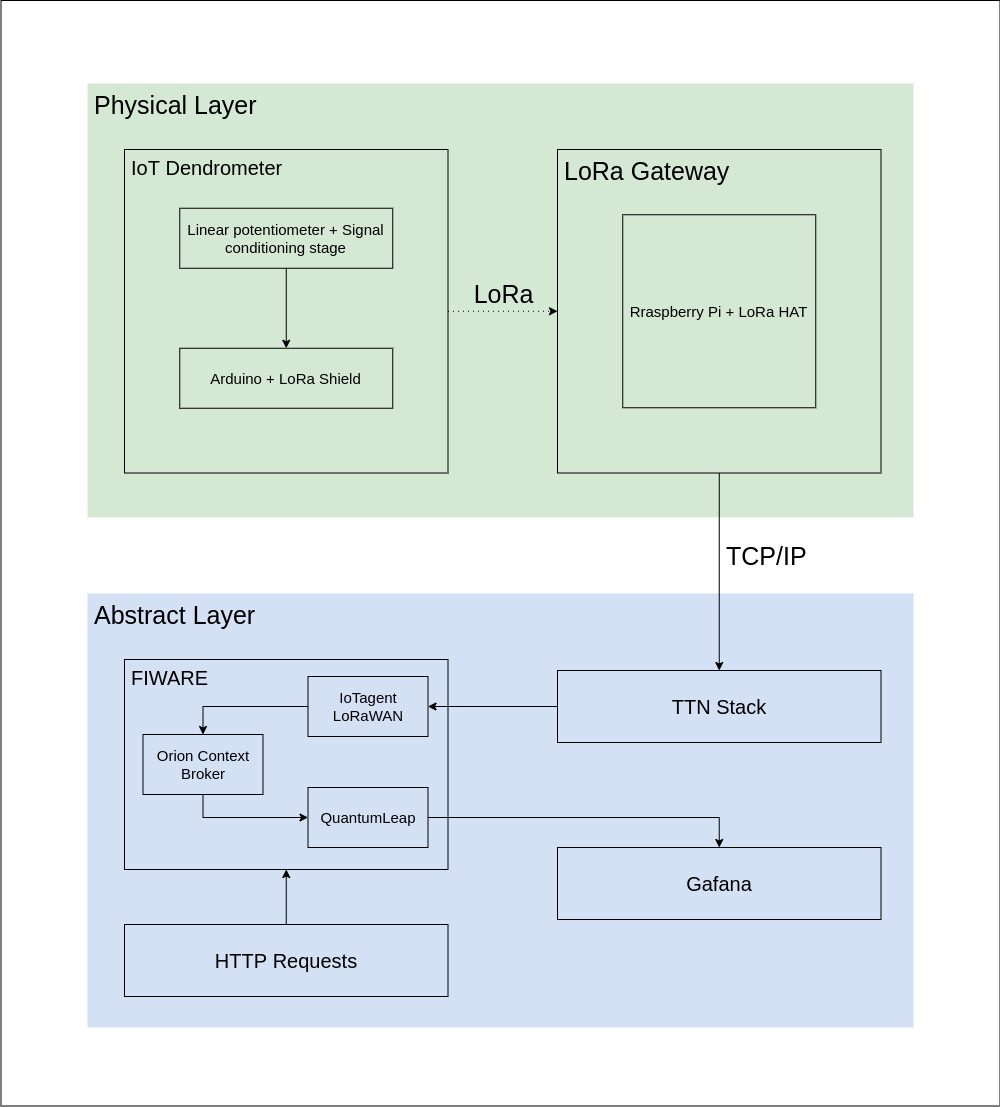
\includegraphics[width=.9\textwidth]{../schemes/simple_scheme_tbg.png}
  \caption{Block diagram overview}
  \label{fig:block_diagram}
\end{figure}

The following subsections will detail each of one. As we can see in figure \ref{fig:block_diagram}, the physical layer is made up of two main modules: the first one is an Arduino microcontroller with its LoRa interface and a linear potentiometer acting as a sensor ---this whole set is the IoT dendrometer--- and a second one consisting of a Raspberry Pi 3b+ with its LoRa interface to act as a gateway.

Meanwhile, the abstract layer is made up of three software modules. TTN stack is a cloud server to retrieve LoRa packets from all existent gateways, FIWARE is a local application server to gather all this context data; and finally Grafana to plot the context data.
\subsection{Physical Layer}

\subsubsection{Arduino, multipurpose microcontroller}
Justifying the use of such an interesting platform as Arduino is not difficult. The adaptability is one of its strengths, therefore; it is able to acquire and process certain data coming from a set of sensors and manage it to send this via any plugged wireless network interface.

Due to circumstances above, an accessible and multipurpose platform to be the basis for the device design itself is needed; i.e. the core part of the dendrometer is an Arduino microcontroller.

Since the idea is to produce a low-cost device in order to distribute a high number of them, it must be a simple design; that's why it consist only of three parts,

\begin{itemize}
  \item \href{https://es.rs-online.com/web/p/products/0317780/}{Linear potentiometer:} which is the sensor itself due to it is directly in contact with the stem. In order to improve data acquisition it will be necessary to use a High Input Impedance Amplifier.
  \item Arduino microcontroller: this is the core part for the device, it will be responsible to acquire linear potentiometer data and send it to a gateway through LoRa interface. 
  \item LoRa interface: similar to other existing wireless interfaces, it is necessary to forward the sensor data to a concentrator (gateway). Usually and due to its complexity these kind of interfaces are integrated circuits which are mounted on a PCB in order to obtain a pluggable card/shield. 
\end{itemize}

% I need to use that \texorpdfstring{}{} for the left-side ToC in PDF viewers, because the ® cannot be rendered in there.
\subsubsection{\texorpdfstring{LoRa\textsuperscript{\textregistered} (Lo{\normalfont\sffamily ng} Ra{\normalfont\sffamily nge})}{LoRa (Long Range)}}
LoRa is a \enquote{long-range, low-power, low-bitrate, wireless telecommunications system}\cite[]{LoRaGeneral}. This is why some devices inside IoT paradigm tend to be economical and low-resources devices, in order to get them distributed/scattered, as it has been pointed. So this low availability (of resources) along with their tendency to be distributed/scattered causes the need for a low-power consumption and a long-range telecommunication.

In a more general sense, there is a wider concept to include all these kind of technologies which fullfil the IoT communication requirements, this is the \enquote{Low-Power Wide Area Networks} (LPWAN), so as claimed by \cite[]{LoRaGeneral}

\begin{quoting}
  Colloquially  speaking,  an LPWAN is supposed to be to the IoT what WiFi was to consumer networking: offering radio coverage over a (very) large area by way of base stations and adapting transmission rates, transmission power, modulation, duty cycles, etc., such that end-devices incur a very low energy consumption due to their being connected.
\end{quoting}

It is important to note that when talking about \enquote{low-power consumption}, in many cases it is actually meaning battery-powered devices.

On the other hand, LoRa can commonly refer to two distinct layers; a physical layer (LoRa itself) and a MAC layer protocol (LoRaWAN). The physical layer, is a proprietary technology developed by Semtech. So it is not fully open; LoRaWAN, however, is a protocol built to use LoRa physical layer, it is intended for sensor networks, wherein those sensors exchange packages with some server with a \enquote{low data rate and relatively long time intervals (one transmission per hour or even days).}\cite[p.~9]{LoRaGeneral}. This particularly means that LoRaWAN protocol is perfect for the purpose of this project.  

\begin{figure}[htp]
  \centering
  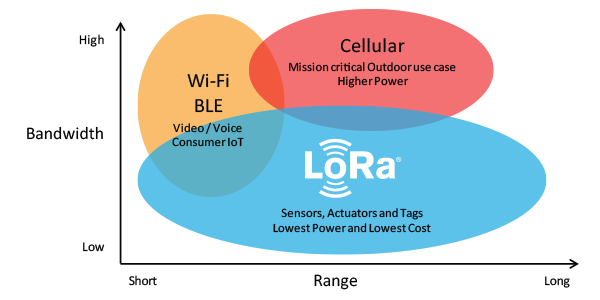
\includegraphics[width=.9\textwidth]{../pictures/LoRa_Why_Range.png}
  \caption{Bandwidth vs range plot for two of the most used telecommunication systems and LoRa.}
  \label{fig:LoraComparison}
\end{figure}

In comparison with other common telecommunication technologies, LoRa uses lower bandwidth, but it reaches longer distances; a comparative diagram shows different wireless technologies in figure \ref{fig:LoraComparison}.
 
\subsubsection{Raspberry Pi, a powerful microcomputer}
As in the case of Arduino, Raspberry Pi provides a powerful platform, however in the case of a Raspberry Pi this platform is slightly more complex than for an Arduino.\footnote{There are a lot of Arduino models, and maybe some of them could be able to support, for example, multiple kind of Real Time Operative Systems, but it is not the case of this project, wherein the Arduino role is just to act as a core for the nodes.} From the hardware perspective, Raspberry Pi implements a better one than Arduino, this also results on a higher cost; however, this hardware allows a Raspberry Pi to support a whole operating system; that's why these devices are usually called \textit{single-board computers}.

A few of interesting hardware specs are for instance, a \textit{Broadcom BCM2837B0, Cortex-A53 (ARMv8) 64-bit SoC @ 1.4GHz} as its CPU, \textit{1GB LPDDR2 SDRAM}, \textit{Gigabit Ethernet over USB 2.0 (maximum throughput 300 Mbps)} or even an \textit{Extended 40-pin GPIO header} among others.\cite{RPiSpecs}

The role for Raspberry Pi in this project is to act like a gateway, receiving all the data from different nodes. So in order to perform this task correctly it is necessary to provide a LoRa interface, which is also embedded (as in Arduino) in a separate pluggable shield/card/hat.

\subsubsection{Dragino shields/hats}\label{sssec:DraginoShields}
These shields/expansion cards are necessary because those devices (Arduino and Raspberry Pi) do not have the ability to comunicate through LoRa physical layer, that's why they need a physical interface in order to manage those LoRa packages. Both shields are based on the SX1276/SX1278 transceiver. However the Raspberry Pi hat also has a L80 GPS interface (Base on MTK MT3339), while Arduino does not.

This project is using the following models: 

\begin{itemize}
  \item \textit{LoRa GPS HAT for Raspberry Pi,}\cite{DraginoRpiHat} which makes use of the extended 40-pin GPIO header to be plugged\footnote{It is important to note this LoRa HAT is not actually designed to play a gateway role, in fact, this is considered a \enquote{Hack where a node-class radio tries to impersonate a gateway}\cite{RpiHatHack}, so this means this hat is designed to be a node-class radio, not a gateway.}
  \item \textit{LoRa Shield for Arduino}\cite{DraginoArdShield}, which is plugged through analog and digital pins.
\end{itemize}

\subsection{Abstract layer}

\subsubsection{The Things Network}
TTN provides a backend system to route the traffic between devices and applications. It is basically a network server placed between gateways and applications servers. It is necessary because LoRaWAN is a non-IP protocol, but a MAC layer protocol and does need some form of routing and processing messages before they can reach the application side. TTN takes care of these steps.

Moreover, this project is based on FIWARE (described in the next subsection) and the LoRaWAN agent in FIWARE is developed to interact with TTN infrastructure, 

\begin{figure}[ht]
  \centering
  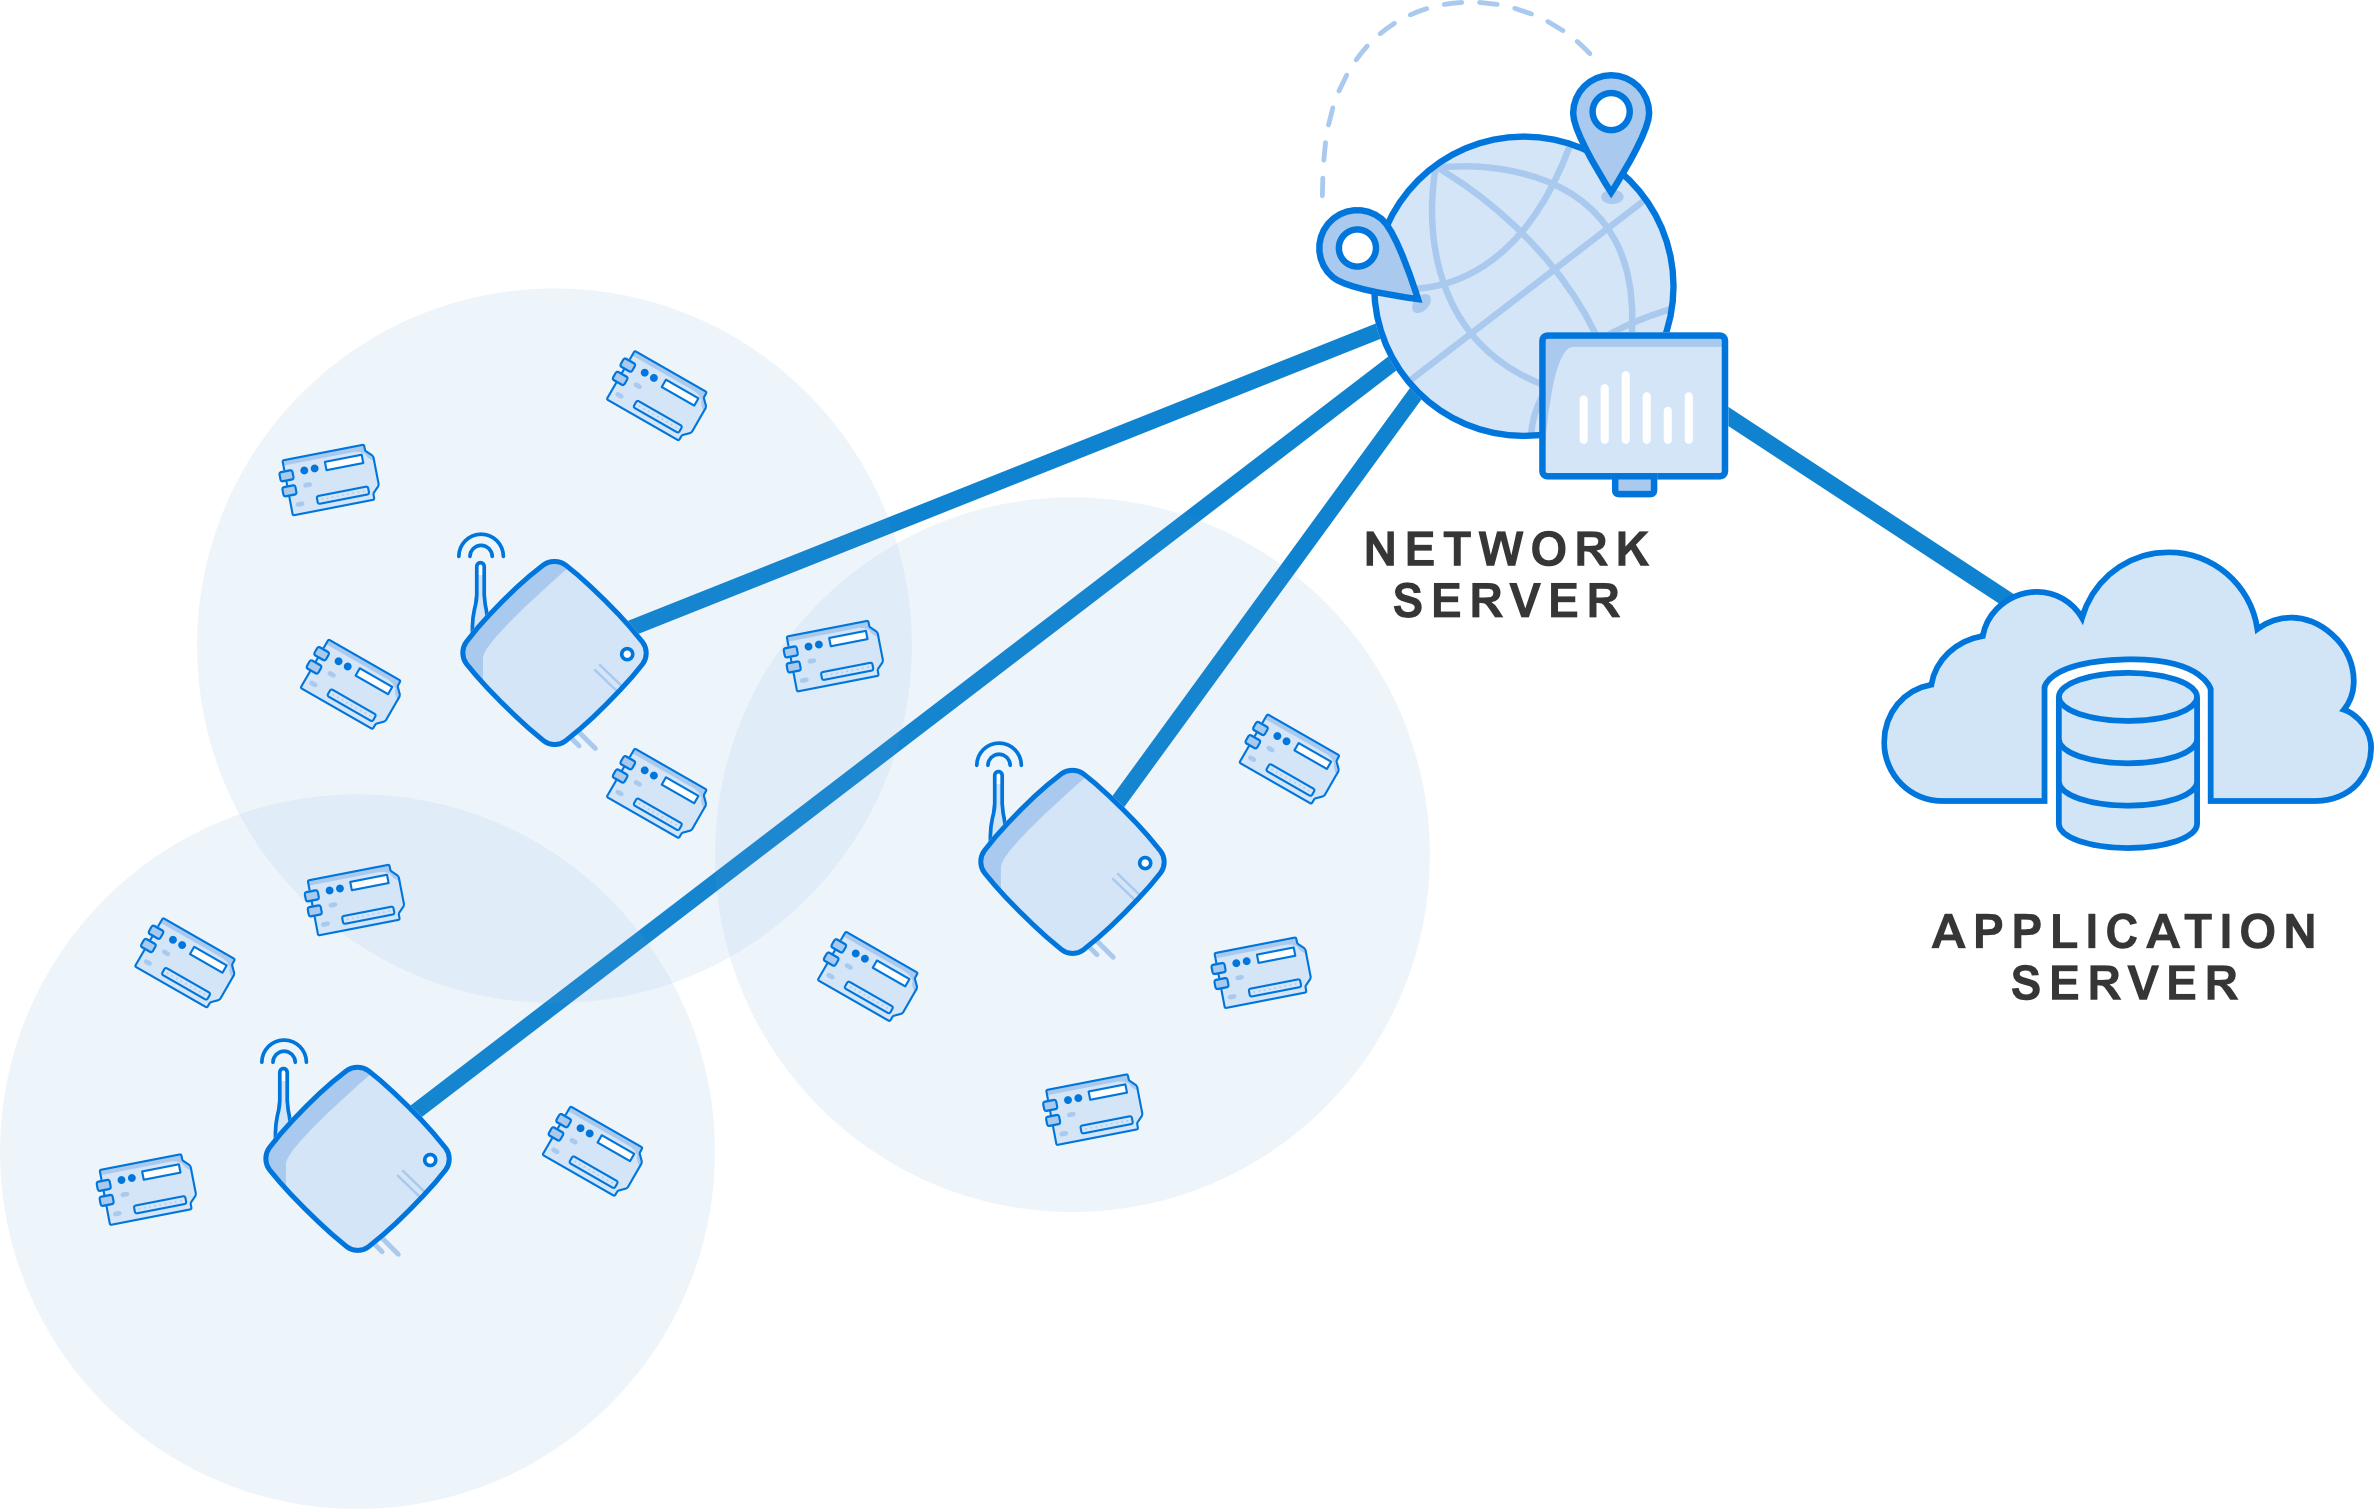
\includegraphics[width=.9\textwidth]{../pictures/TTN_overview.png}
  \caption{TTN basic diagram.}
  \label{fig:TTN_overview}
\end{figure}

End-node devices broadcast LoRaWAN packets over LoRa radio protocol to the gateways, these gateways will forward these packets to the TTN backend, where a software module called Router will manage the gateway status and schedule transmissions. These routers are connected to other software modules called Brokers, that are responsible for mapping a device to an application ---into TTN environment--- allowing downlink and uplink transmissions. Once these uplink transmissions are inside TTN environment, the FIWARE LoRaWAN agent will retrieve them, however this is actually the application server shown in figure \ref{fig:TTN_overview}. \enquote{The goal of The Things Network is to be very flexible in terms of deployment options.} \cite{TTN_net_arch}. As explained in the docs, TTN infrastructure provides different \enquote{core functions} divided in four main groups:

\begin{itemize}
  \item Gateway-related functions, in order to schedule and manage the gateways.
  \item Device-related functions, to manage the state and received context data from specific devices.
  \item Application-related functions, to group different devices used for similar purposes.
  \item Service discovery functionality, which helps components to determine where traffic should be routed to. 
\end{itemize}

After this, the traffic is routed to FIWARE side, which is deployed locally and the user has total control over it.

\subsubsection{FIWARE}
FIWARE is defined as \enquote{The Open Source Platform for Our Smart Digital Future}\cite{FIWARE}; in a deeper sense it is \enquote{an open source initiative defending an universal set of standards for context data management}\cite{FIWARE}, which basically means that \textit{FIWARE} is an open source platform where IoT and smart solutions can be developed. The platform provides a number of software modules called \textit{Generic Enablers}; among all those \textit{Generic Enablers} there is one particularly important called \textit{Orion Context Broker}. In fact, for a solution to be considered as \textit{Powered by FIWARE} it must to use the \textit{Orion Context Broker} at least. 

This \textit{Context data} is just a way to name any kind of data coming from any kind of sensor. \textit{Orion Context Broker} is designed to manage this context data through concepts such as \textit{subscriptions} or \textit{entities}, to name but a few; however, all these \textit{Generics Enablers} communicate with each other using the \textit{FIWARE NGSI RESTful API}\cite{NGSI}.\footnote{\textit{RESTful} term comes from the software architectural style \textit{REST}, which stands for \textit{Representational State Transfer}}

\subsubsection{Simple Graphical Interface}
Despite FIWARE is a powerful platform, is not friendly enough regarding final user. This is why a the end of this document is described a simple graphical interface developed to manage end-nodes in FIWARE side. As will be indicated, this graphical interface has been developed using python and its tkinter module intended to build graphical interfaces.

There are a lot of HTTP clients available, however the reader would be still forced to make manually these HTTP requests, these could result a little complex for a non advanced user, that's why this graphical interface has been developed.

It's not perfect, it has a few deficiencies in fact, but is by the moment an appropriate way to manage devices, entities and subscriptions in locally deployed FIWARE instance. \href{https://github.com/WyRe/lora-arduino-dendrometer/blob/master/src/api-gui/api-gui.py}{The code} of this graphical interface is available in the project repository at GitHub.

\clearpage{\pagestyle{empty}\cleardoublepage}\thispagestyle{plain} % Forces the next section to start in an odd page.
\section{Design}\thispagestyle{plain}
Like in the Introduction, the most proper way to present this technical description is to difference between software and hardware parts. However, is still interesting to present a simple and general diagram for whole designed solution. So as the reader can see in the figure \ref{fig:GenView} is shown the general diagram. 

Firstly the TTN stack send through MQTT protocol the payload to FIWARE IoTagent-LoRaWAN generic enabler. Secondly, FIWARE generic enablers process that payload and store the contained information (also called \textit{context data}) along with a timestamp in the persisting data base (CrateDB), after this, the context data can be visualized in a web view provided by Grafena. 

At this moment this solution requires to send manually the HTTP requests in order to communicate with FIWARE generic enablers manually. The ideal situation would be to develop a desktop or web application capable of provide any kind of graphical user interface to easily set up the two most important requirements to get the solution working as intended ---Create a new device using the IoTagent-LoRaWAN, create a subscription in Orion Context Broker which sends notifications to QuantumLeap.

\begin{figure}[htp]
  \centering
  
\includegraphics[width=\textwidth]{../schemes/main_scheme_tbg.png}
  \caption{General view of this solution.}
  \label{fig:GenView}
\end{figure}

\subsection{Hardware}

\subsubsection{Nodes}
Nodes are the parts of the system in direct contact with trees themselves (one node per each tree). Most important features in those devices are: low-cost, low-powered, wireless communication and small size. The figure \ref{fig:NodeDiag} shows a diagram of its most relevant parts:

\begin{figure}[htp]
  \centering
  
\includegraphics[width=.9\textwidth]{../schemes/node_tbg.png}
  \caption{Diagram for a detailed view of a node.}
  \label{fig:NodeDiag}
\end{figure}

This diagram shows three different parts:

\begin{itemize}
  \item A linear potentiometer, ideally an \href{https://docs.rs-online.com/37bf/0900766b814f0bd0.pdf}{RS Pro Conductive Polymer
  Potentiometer for Automotive Applications}, however, by circumstances is not possible to use it and in order to perform a kind of proof of concept, this project will implement a regular rotary potentiometer.
  \item A signal conditioning stage, which is needed in order to improve the quality of the voltage signal produced by the potentiometer.
  \item Arduino + Dragino LoRa Shield; of course it is necessary to schedule data transmission and acquisition, as well as transmit them using the LoRa physical layer and LoRaWAN protocol. For this purpose an Arduino-like microcontroller is perfect.
\end{itemize}

\subsubsubsection{Linear Potentiometer}
As said, ideally this potentiometer should be a linear potentiometer with $5\ \si{\kilo\ohm}$ of maximum resistance, however, in order to improve its performance, it's recommended to use it as a voltage divider; also it would be convenient to buffer the resulting output with a high impedance amplifier, that's why the figure \ref{fig:NodeDiag} includes a signal conditioning stage, which will be described below.

\subsubsubsection{Signal conditioning}
This stage is focused on improve the signal acquisition, according to this potentiometer specifications, the best way to achieve this objetive is using a high input amplifier, in fact, a single-supply, rail-to-rail operational amplifier is the best option. \doubt{Figure \ref{fig:SignalCond} shows a possible schematics for this stage.}

It is also recommended by the manufacturer to use the potentiometer as a voltage divider instead a variable resistor, this is why taking advantage of the Arduino power source, particularly the 5 \si{\volt} and GND pins.

\begin{figure}[htp]
  \centering
    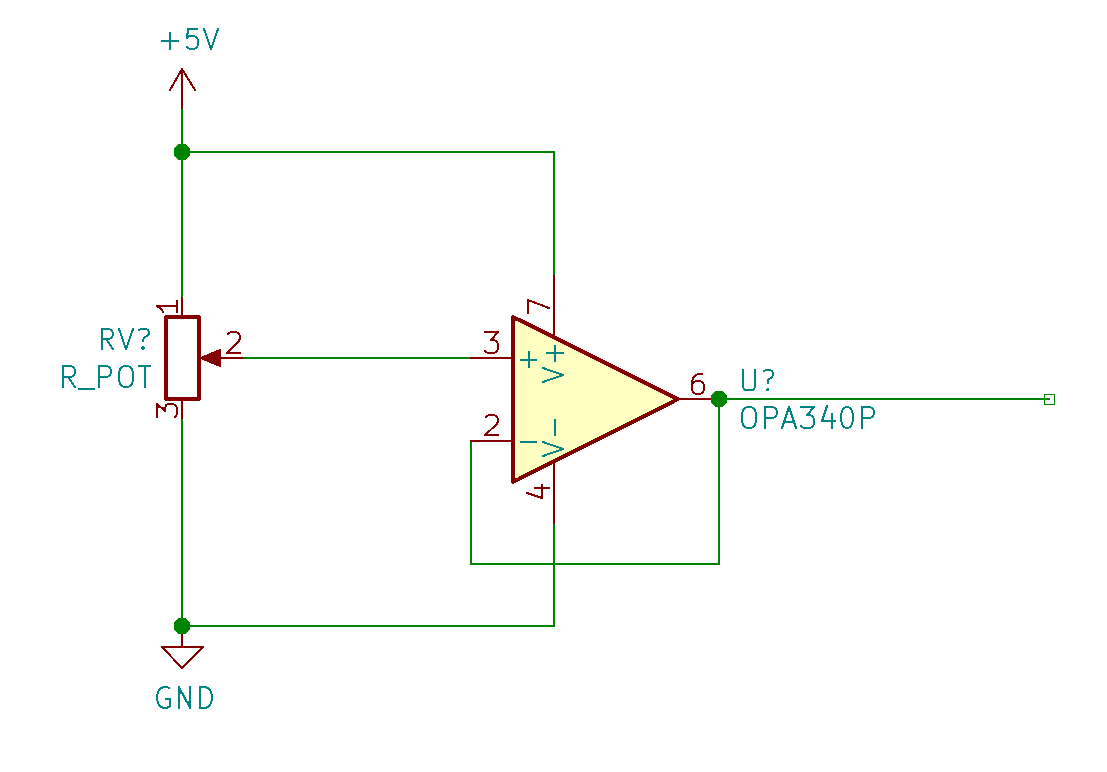
\includegraphics[width=.9\textwidth]{../schemes/Signal_Conditioning.png}
  \caption{Signal conditioning stage.}
  \label{fig:SignalCond}
\end{figure}

\subsubsubsection{Arduino}
In a first place, \href{https://github.com/WyRe/lora-arduino-dendrometer/blob/master/src/arduino/dendro/dendro.ino}{the sketch} can be found in \cmd{src/dendro/dendro.ino} path. This is the sketch that must be uploaded to arduino microcontroller. MEGA 2560 in this case.

On the other hand, in order to this sketch takes advantage of the plugged LoRa Shield, is required to base it on the LoRaMAC-in-C library \cite{MCCI_lmic} (\cmd{arduino-lmic})\footnote{Dragino has its own \href{https://github.com/dragino/arduino-lmic}{fork of this library} but has been considered less upgraded than the MCCI version, which is a fork itself from the first port of LMIC library by \href{https://github.com/matthijskooijman}{Matthijs Kooijman}.} implemented by \href{https://mcci.com/}{MCCI}, whose technical documentation can be found in \cite{MCCI_lmic_docs}. The \cmd{arduino-lmic} library is, as its description in the README.md says, a port from the IBM LoRaWAN MAC in C, but \enquote{slightly modified to run in the Arduino environment allowing using the SX1272, SX1276 transceivers and compatible modules} \cite{MCCI_lmic}. The original IBM LoRaWAN MAC in C library was developed for microcontrollers in general, their examples and HAL ---Hardware Abstraction Layer or rather Hardware Annotation Library--- were only for STM32 MCUs (but bare-metal, so no Arduino on top). 

There is an \textit{Arduino-like wrapper} library called \href{https://github.com/mcci-catena/arduino-lorawan}{\cmd{arduino-lorawan}} also developed by MCCI; this library provides apparently a higher abstraction level and it could be helpful in a future to keep growing this project, however, for now this project is implemented using the mentioned \cmd{arduino-lmic}.

Basically the sketch is based on the \href{https://github.com/mcci-catena/arduino-lmic/blob/master/examples/ttn-abp/ttn-abp.ino}{ttn-abp example}, as the reader can see in the first comment block; that example sends a LoRaWAN valid package with the payload \enquote{Hello World!}. Besides it uses the ABP (Activation-by-personalization) method ---in opposition to OTAA (Over-the-air-activation) method---, depending on the used method it is necessary to include different security keys provided by The Things Network stack (TTN stack) in the code \cite{TTN_Security}. \textbf{It is important to note that frame counters in TTN console must be reset every time the device is reset, powered off or flashed again} \cite{TTN_frame_counters}.

As commented \href{https://github.com/mcci-catena/arduino-lmic/blob/master/examples/ttn-abp/ttn-abp.ino#L29}{lines 29 and 30} point, the most important thing before start working on the sketch is to configure the \cmd{arduino-lmic} library, so after install the library with the library manager ---in the Arduino IDE or any other chosen IDE---, the reader will need to go the library path and locate the \href{https://github.com/mcci-catena/arduino-lmic/blob/master/project_config/lmic_project_config.h}{\cmd{<lib\_path>/project\_config/lmic\_project\_config.h}} file to ensure the line 2 (\cmd{\#define CFG\_eu868 1}) is \textbf{uncommented} and the line 3 (\cmd{\#define CFG\_us915 1}) is \textbf{commented}. This is to enable specific functions in the library for Europe region (where the radio regulations are slightly different than in other regions); so this \cmd{lmic\_project\_config.h} must looks like in te example \ref{ej:lmic_project_config.h}

\begin{lstlisting}[%
  % float=ht,
  language=cpp,
  firstnumber=1,
  caption={Configuring lmic library radio.},
  label=ej:lmic_project_config.h
  ]
  // project-specific definitions
  #define CFG_eu868 1
  //#define CFG_us915 1
  //#define CFG_au915 1
  //#define CFG_as923 1
  // #define LMIC_COUNTRY_CODE LMIC_COUNTRY_CODE_JP	/* for as923-JP */
  //#define CFG_kr920 1
  //#define CFG_in866 1
  #define CFG_sx1276_radio 1
  //#define LMIC_USE_INTERRUPTS
\end{lstlisting}

After this, the sketch may use specific functions to perform radio transmissions in Europe region. This in fact, will has an impact in the \cmd{void setup()\{\}} function ---in the example sketch ttn-abp--- so lines between \href{https://github.com/mcci-catena/arduino-lmic/blob/master/examples/ttn-abp/ttn-abp.ino#L232}{line 232} and line 254 will be executed when the library is configured for Europe region.

Once the library has been properly configured, the second most important thing is set the pin mapping for the chip, according to the \href{https://github.com/mcci-catena/arduino-lmic#pin-mapping}{Pin Mapping section} in the \cmd{README.md}, \enquote{a variety of configurations are possible}. Then, the most appropriate way to make the pin mapping is following the Dragino indications, so following the figure \ref{fig:Ard_LoRa_Shield_pin_mapping} ---which can also be found in \href{http://wiki.dragino.com/index.php?title=Lora_Shield#Pin_Mapping_and_Unused_Pins}{Dragino documentation}.

\begin{figure}[ht]
  \centering
  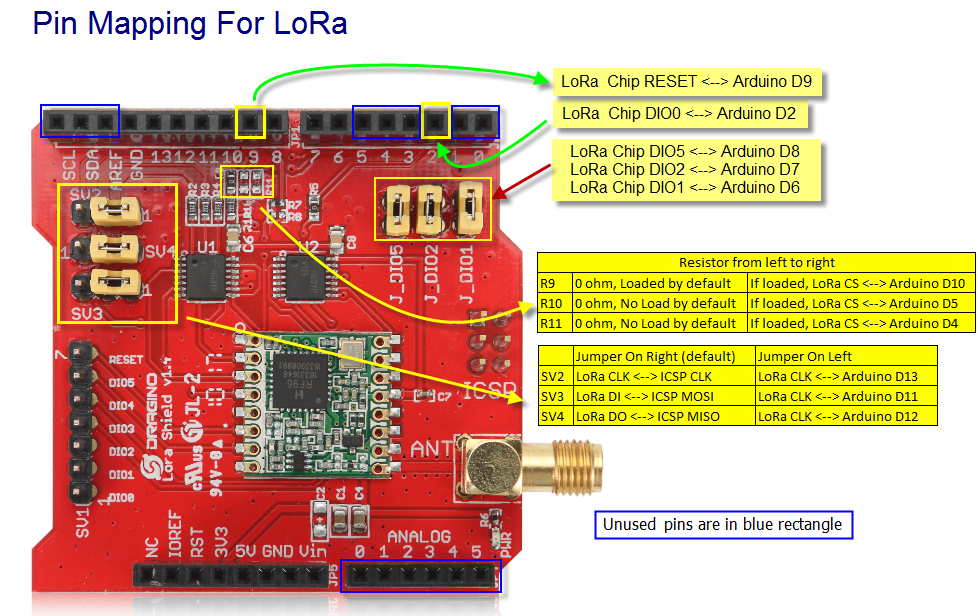
\includegraphics[width=.9\textwidth]{../pictures/LoRa_Shield_Pin_Mapping.png}
  \caption{Arduino LoRa Shield pin mapping.}
  \label{fig:Ard_LoRa_Shield_pin_mapping}
\end{figure}

The reader can see the LoRa Chip reset pin is \cmd{D9} and as DIO pins ---Digital Input/Output--- the board has assigned \cmd{D2} to DIO0, \cmd{D6} to DIO1, \cmd{D7} to DIO2. Besides, a brand new board will only have loaded the \cmd{R9} resistor, this means the LoRa CS pin will be the \cmd{D10}. This leads to set the pin mapping shown in example \ref{ej:pin_mapping}

\begin{lstlisting}[%
  % float=ht,
  language=cpp,
  firstnumber=77,
  caption={Pin mapping for this Dragino LoRa Shield.},
  label=ej:pin_mapping
  ]
  // Pin mapping
  const lmic_pinmap lmic_pins = {
    .nss = 10,
    .rxtx = LMIC_UNUSED_PIN,
    .rst = 9,
    .dio = {2, 6, 7},
  };
\end{lstlisting}

On the other hand \enquote{Any pins that are not needed should be specified as \cmd{LMIC\_UNUSED\_PIN}} as it can be also read in the \href{https://github.com/mcci-catena/arduino-lmic#pin-mapping}{Pin Mapping section} of the library \cmd{README.md}. As the reader can see, the example \ref{ej:pin_mapping} starts at line 76, that is because this is the line where the pin mapping is placed in the \href{https://github.com/WyRe/lora-arduino-dendrometer/blob/master/src/arduino/dendro/dendro.ino#L76}{written sketch}.

With regards to LoRaWAN and TTN security, as previously indicated, the chosen method is ABP, so are necessary the \cmd{NWKSKEY} (Network Session Key), \cmd{APPSKEY} (Application Session Key) and \cmd{DEVADDR} (End-Device Address); these constants placed at lines \href{https://github.com/WyRe/lora-arduino-dendrometer/blob/master/src/arduino/dendro/dendro.ino#L48}{48}, \href{https://github.com/WyRe/lora-arduino-dendrometer/blob/master/src/arduino/dendro/dendro.ino#L52}{52} and \href{https://github.com/WyRe/lora-arduino-dendrometer/blob/master/src/arduino/dendro/dendro.ino#L57}{57} must be obtained from TTN console as will be explained in \hyperref[sssec:TTN_Stack]{The Things Network Stack} subsection, so \textbf{pleas, refer to that subsection for further details}. The sketch also sets analog pin \cmd{A2} to acquire the sensor signal as it can be seen in line \href{https://github.com/WyRe/lora-arduino-dendrometer/blob/master/src/arduino/dendro/dendro.ino#L70}{70}.% as well as the payload to send through LoRa interface in line \href{https://github.com/WyRe/lora-arduino-dendrometer/blob/master/src/arduino/dendro/dendro.ino#L65}{65}

\begin{lstlisting}[%
  % float=ht,
  language=cpp,
  firstnumber=69,
  caption={Variables for the potentiometer signal acquisition.},
  label=ej:potmeter_vars
  ]
  // Potentiometer pins
  int potPin = A2;               // Potmeter pin
  double potVal = 0;             // Potmeter value
\end{lstlisting}

Finally, the reader can find the core of this sketch inside \cmd{void do\_send(osjob\_t* j)\{\}} function, at line \href{https://github.com/WyRe/lora-arduino-dendrometer/blob/master/src/arduino/dendro/dendro.ino#L176}{176}; here the reader can find the following lines of code

\begin{lstlisting}[%
  % float=ht,
  language=cpp,
  firstnumber=181,
  caption={Prpareing the payload.},
  label=ej:prep_payload
  ]
  // Prepare upstream data transmission.
        
  // Read the analog value of the potmeter (0-1023)
  potVal = analogRead(potPin);
  potVal = 100.0 * potVal / 1023;
  
  // Write the value to the serial monitor
  Serial.println(potVal);
         
  // Reset CayenneLPP buffer
  lpp.reset();

  // Add the measured value to CayenneLPP buffer
  lpp.addAnalogInput(1, potVal);

  // prepare upstream data transmission at the next possible time.
  // transmit on port 1 (the first parameter); you can use any value from 1 to 223 (others are reserved).
  // don't request an ack (the last parameter, if not zero, requests an ack from the network).
  // Remember, acks consume a lot of network resources; don't ask for an ack unless you really need it.
  LMIC_setTxData2(1, lpp.getBuffer(), lpp.getSize(), 0);
  Serial.println(F("Packet queued"));
\end{lstlisting}

So, as it can be seen, in order to prepare the payload firstly the sketch reads the analog pin and stores the read value in \cmd{potVal} variable ---which is a \cmd{double} type and this makes no difference with \cmd{float} type \enquote{On the Uno and other ATMEGA based boards} but it makes \enquote{On the Arduino Due} \cite{Ard_double_type}; after this the function \cmd{lpp.reset()} is used to reset the CayenneLPP buffer, then the measure \cmd{potVal} is added to the CayenneLPP buffer in the first channel using the function \cmd{lpp.addAnalogInput()}, finally the buffer content is prepared to be transmitted at the next possible time using the function \cmd{LMIC\_setTxData2()}. 

These \cmd{lpp.*()} functions are part of the CayenneLPP library \cite{CayenneLPP_lib} ---which is also dependent of ArduinoJson library \cite{ArduinoJson_lib}; in particular, the \cmd{lpp.addAnalogInput()} function encodes the raw value as a number encoded in 2 bytes (16 bits signed) with a unit of 0.01. In 16 bits signed is possible to represent numbers from -32768 until 32767, so with a unit of 0.01, that amounts to a range from -327.68 to +327.67; that is because the sketch includes the line \href{https://github.com/WyRe/lora-arduino-dendrometer/blob/master/src/arduino/dendro/dendro.ino#L185}{185}, where the raw value \cmd{potVal} is scaled to a [0, 100.0] range. This range will fit in the range that can be encoded in CayenneLPP. 

CayenneLPP is so important because FIWARE will work with this data model, so any other third party encoding will not be admitted/decoded by the FIWARE LoRaWAN agent.

It is also important to note that, as will be stated in \hyperlink{Raspi_HAT}{2.1.2.2 Dragino GPS and LoRa HAT} subsection, the SX1276 is a single channel chip and only can listen in one channel, so despite inside \cmd{void setup()} function the channels are set up as shows the example \ref{ej:chan_setup}, the gateway only will be able to listen the channel 0 (868.1 \si{\mega\hertz}), which is the frequency set in \href{https://github.com/dragino/dual_chan_pkt_fwd/blob/master/global_conf.json}{global\_conf.json} at \cite{Dragino_DualChannelController_Rpi}

\begin{lstlisting}[%
  % float=ht,
  language=cpp,
  firstnumber=251,
  caption={Channels setup.},
  label=ej:chan_setup
  ]
  LMIC_setupChannel(0, 868100000, DR_RANGE_MAP(DR_SF12, DR_SF7),  BAND_CENTI);  // g-band
  LMIC_setupChannel(1, 868300000, DR_RANGE_MAP(DR_SF12, DR_SF7B), BAND_CENTI);  // g-band
  LMIC_setupChannel(2, 868500000, DR_RANGE_MAP(DR_SF12, DR_SF7),  BAND_CENTI);  // g-band
  LMIC_setupChannel(3, 867100000, DR_RANGE_MAP(DR_SF12, DR_SF7),  BAND_CENTI);  // g-band
  LMIC_setupChannel(4, 867300000, DR_RANGE_MAP(DR_SF12, DR_SF7),  BAND_CENTI);  // g-band
  LMIC_setupChannel(5, 867500000, DR_RANGE_MAP(DR_SF12, DR_SF7),  BAND_CENTI);  // g-band
  LMIC_setupChannel(6, 867700000, DR_RANGE_MAP(DR_SF12, DR_SF7),  BAND_CENTI);  // g-band
  LMIC_setupChannel(7, 867900000, DR_RANGE_MAP(DR_SF12, DR_SF7),  BAND_CENTI);  // g-band
  LMIC_setupChannel(8, 868800000, DR_RANGE_MAP(DR_FSK,  DR_FSK),  BAND_MILLI);  // g2-band
\end{lstlisting}

Because of explained above, the gateway will just receive one package per each $\sim$10 minutes ---at line 74 in the sketch the transmission interval is set at 60 seconds, so as there are 9 channels but the gateway is just listening the channel 0, the microcontroller is transmitting at this channel once in 9---

\begin{lstlisting}[%
  % float=ht,
  language=cpp,
  firstnumber=73,
  caption={Transmission interval.},
  label=ej:tx_interval
  ]
  // Schedule TX every this many seconds (might become longer due to duty
  // cycle limitations).
  const unsigned TX_INTERVAL = 60;
\end{lstlisting}

Of course this parameter can be adjusted, but for the final purpose of this project 60 seconds are even too many, in order to monitor changes in stem diameter of a tree, a more appropriate value would be 3600 seconds (1 hour) or even greater.  

\subsubsection{Gateway}\label{sssec:Gateway}

\subsubsubsection{Raspberry Pi 3 B+}
This model of Raspberry Pi is able to run almost every GNU/Linux distribution ported to ARM architecture, Raspberry Pi OS, formerly known as Raspbian, \cite{RaspberryPiOs} is in fact a Debian port to ARM architecture. After a little researching, it is possible to conclude that there is not other operative system which improves the performance of Raspberry Pi OS in a Raspberry Pi. Due to this former argument this project is going to use Raspberry Pi OS.

One of the most interesting features of Raspberry Pi is precisely that OS is installed and run from a microSD card, so the hardware is loading the operative system from this microSD card to the RAM directly, which improves notably the system load times, and increments its portability.

Raspberry Pi foundation provides the \href{https://www.raspberrypi.org/downloads/noobs/}{\textit{Raspberry Pi Imager}} to perform the installation in a microSD card.\footnote{There are many ways to perform the Raspberry Pi OS installation in a microSD card, this document leaves it to readers to use their preferred method. However, this document also considers the \textit{Raspberry Pi Imager} method as the best one.} This tool allows the reader to choose between three different versions of Raspberry Pi OS. Recommended, Lite and Full version. Lite version is the same than Recommended version but without graphical user interface (GUI or Desktop Environment), meanwhile Full version is the same than Recommended version but with a few extra applications.

This project is using the Recommended version for Raspberry Pi OS, nevertheless, the project does not require absolutely the desktop environment, so to maximize the available free space in the SD card, is better to install the Lite version instead of the Recommended version.

\begin{figure}[htp]
  \centering
  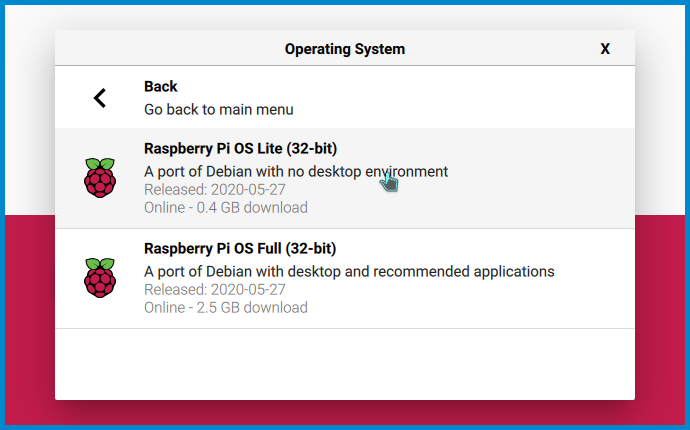
\includegraphics[width=.9\textwidth]{../pictures/rpi_imager.png}
  \caption{Raspberry Pi Imager showing different options to install Raspberry Pi OS in a microSD card.}
  \label{fig:RpiImager}
\end{figure}

Even so, independently of the installed version, the reader will be able to disable the graphical environment using the console based \cmd{raspi-config} application \cite{RaspiConf}. 

One of the first and most important configurations is the internet access; this can be done via two different ways, using the ethernet port (which does not require any extra configuration, just tu plug the cable) or using the WiFi interface, which can be configured using also \cmd{raspi-config} \cite{RaspiWIFIcli}. Due to its versatility, there are multiple setup that could fulfil the requirements of this projects:

\begin{itemize}
  \item \textbf{PoE} (Power-over-Ethernet); this is not actually a suitable option because Raspberry Pi does not support PoE by itself, it needs a \href{https://www.raspberrypi.org/products/poe-hat/}{separate HAT} which is using the GPIO connector, so this makes impossible to use it along the LoRa HAT. Apparently there are hacks to reduce this HAT size, but they also use pins in the GPIO connector \cite{RaspiPoEHack}. Besides, this method only works with up to 100m cables, so it would be necessary to have a power source and internet access point within a 100m radius.\footnote{The \href{https://github.com/hallard/LoRasPI}{LoRasPI HAT} is more suitable for this option because does not cover whole GPIO connector, leaving free the GPIO pins used in \cite{RaspiPoEHack}.}
  \item \textbf{WiFi} and battery powered; this setup implies also the existence of a relatively close power source, because the access point used to provide that wireless network connection should work also with mains power. Probably the WiFi radio is not enough to make it the difference between this setup and the next one suggested.
  \item Simple \textbf{ethernet} and mains power, this setup is similar to the previous one exposed, but omitting the WiFi limitations/configurations, the access point and the Raspberry Pi should be practically both at the same location.
  \item \textbf{GSM module} and battery or mains powered; this document consider this as the ideal setup. This setup doesn't require a conventional access point because the internet access is granted through a GSM module, in a similar way than a mobile phone. This would be the ideal way because it minimizes the resources needed, which is crucial in an environment where those probably won't be available ---in the middle of the forest.
  
  Furthermore, this is apparently possible through two different options:
    \begin{itemize}
      \item \href{https://www.itead.cc/wiki/RPI_SIM800_GSM/GPRS_ADD-ON_V2.0}{Itead Raspberry Pi GSM Board (SIM800)}. This is not the most interesting way, because though GPIO pins comes through this does mean the HAT supports \href{http://www.pi-in-the-sky.com/index.php?id=stacking-guide}{stacking}, and even if that does, doesn't mean every other HAT would.
      \item \href{https://tutorials-raspberrypi.com/raspberry-pi-gsm-module-mobile-internet-lte-3g-umts/}{USB GSM module}. This is apparently the most promising option. These kind of GSM modules are in general compliant with GNU/Linux systems and using a regular SIM card, they would be eventually able to provide an internet access point. Of course, this also will to increment the size of the whole device.
    \end{itemize}
\end{itemize}

It is important to note the need for a relatively stable internet connection; those gateways will forward the traffic to the cloud server, so they are receiving LoRa packets through its LoRa interface and then forwarding them to the specified server. 

Another configuration which must be done is the Secure Shell (\cmd{ssh}) service; which according to Raspberry Pi documentation can be done from terminal using \cmd{systemd} \cite{RaspiSSH}. 

So generating a pair of keys and configuring properly the ssh access;\footnote{The reader will probably need to figure out the Raspberry IP in their local network, otherwise, inside a local network will not be necessary specify any port for ssh, though it usually is the 22 by default.} it will probably be necessary to paste the \cmd{*.pub} key content into \cmd{~/.ssh/authorized\_keys} file (located in the local folder in the Raspberry Pi); and give it the right permissions (\cmd{700}), after this the reader should be able to connect through ssh service.

\begin{lstlisting}[%
    % float=ht,
    language=json,
    firstnumber=1,
    caption={Creating a pair of ssh keys.},
    label=ej:CreateEntity
    ]
    $ ssh-keygen
    Generating public/private rsa key pair.
    Enter file in which to save the key (/home/wyre/.ssh/id_rsa): 
    Enter passphrase (empty for no passphrase): 
    Enter same passphrase again: 
    Your identification has been saved in /home/wyre/.ssh/id_rsa
    Your public key has been saved in /home/wyre/.ssh/id_rsa.pub
    The key fingerprint is:
    SHA256:vkNRk/Fo8iGGo0pYlwb2L3vf3TgOfm11MmZW+BipXgQ wyre@DESKTOP-AFG84JJ
    The key's randomart image is:
    +---[RSA 3072]----+
    |  o       .o     |
    | . o . .  +oE    |
    |  . = o +.+... o |
    | o o o o.= .  = .|
    |. . o . S..  o = |
    | . . o ..   . O +|
    |  . . ... .. * +.|
    |     . ..+ o+oo  |
    |        o.oo+o.  |
    +----[SHA256]-----+
\end{lstlisting}

Once is available the remote control for Raspberry Pi through ssh, is possible to manage it completely from the command line, even upgrade the system and compile the required controller to get properly working the LoRa transceiver. 

At this point and depending on the type of access point used to provide internet service to the Raspberry, the reader will be able even to remote control the Raspberry over internet. For this purpose could be useful to read the access point documentation in order to perform port forwarding or alternatively \href{http://www.thirdway.ch/En/projects/raspberry_pi_3g/index.php}{a reverse tunnel over ssh} ---in the case the ISP does not allow ssh when using a GSM module, also the reader may find that IPv6 works but IPv4 does not. Anyway, as said the internet access point could be variable and it is not determined by this project.\footnote{The most important thing is to work comfortably with the Raspberry Pi with no HDMI, keyboard and mouse plugged, and this can be done locally in a LAN to configure it in a first place.}  

\subsubsubsection{Dragino GPS and LoRa HAT}
Gateways doesn't need actually a diagram or detailed description because there are multiple devices which could play this role. These usually are generic devices due to LoRaWAN protocol versatility. LoRaWAN is a cloud-based medium access control (MAC) layer protocol, but actually acts as a network layer protocol for managing communication between gateways and nodes, similar to a routing protocol. So it is possible for any device which implements hardware for a LoRa physical layer, to act as a gateway.

Nevertheless, there are important considerations about the said above, for example, nodes are not actually associated with an specific gateway. Instead, data transmitted by a node is typically received by multiple gateways. Each gateway will forward the received packets from the end-node to de cloud-based network server. Besides, this project is using a Raspberry Pi 3B+ with a Dragino Hat which mounts a SX1276 LoRa \textbf{transceiver}\cite{SX1276}; this is so important because means, according to Semtech, this transceiver is not intended to play a gateway role, but a end-node role.

A transceiver, by definition, is a device that is able to both, transmit and receive (in fact, the word itself is a mix between both, \textbf{trans}miter and re\textbf{ceiver}) that is what a node must be able to do; i.e. transmit the sensor data (context) and receive data to perform operations with its actuators. 

Nevertheless, LoRaWAN specification varies from region to region \enquote{based on
the different regional spectrum allocations and regulatory requirements}\cite[p.~12]{LoRaWANspec}. In fact, for Europe, and again as reported by \cite[p.~13]{LoRaWANspec} 

\begin{quoting}
LoRaWAN defines ten channels, eight of which are multi data rate from 250bps to
5.5 kbps, a single high data rate LoRa channel at 11kbps, and a single FSK channel
at 50kbps.
\end{quoting}

\hypertarget{Raspi_HAT}{Here} is the important point. This Dragino HAT for the Raspberry Pi, mounts an SX1276 transceiver, which is known as node-class transceiver, so in conclusion, \textbf{this Dragino LoRa GPS HAT is LoRaWAN compatible but isn't LoRaWAN compliant}. The main reason the SX1276 transceiver is not suitable to work as a gateway is that \textbf{it is actually a single channel transceiver}. Despite all of this, there still exist the possibility of use it as a gateway, because it is technically possible.


Dragino foresees this and provides a dual channel controller \cite{Dragino_DualChannelController_Rpi}. The most important thing about this dual channel controller, is not the possibility to use the transceiver in a dual channel mode, but to use it as a gateway in the physical sense.

In order to get the HAT operative, the reader will need to enable the SPI (Serial Peripheral Interface). This can be done also with \cmd{raspi-config} like shows the figure \ref{fig:EnablingSPI} 

\begin{figure}[ht]
  \centering
  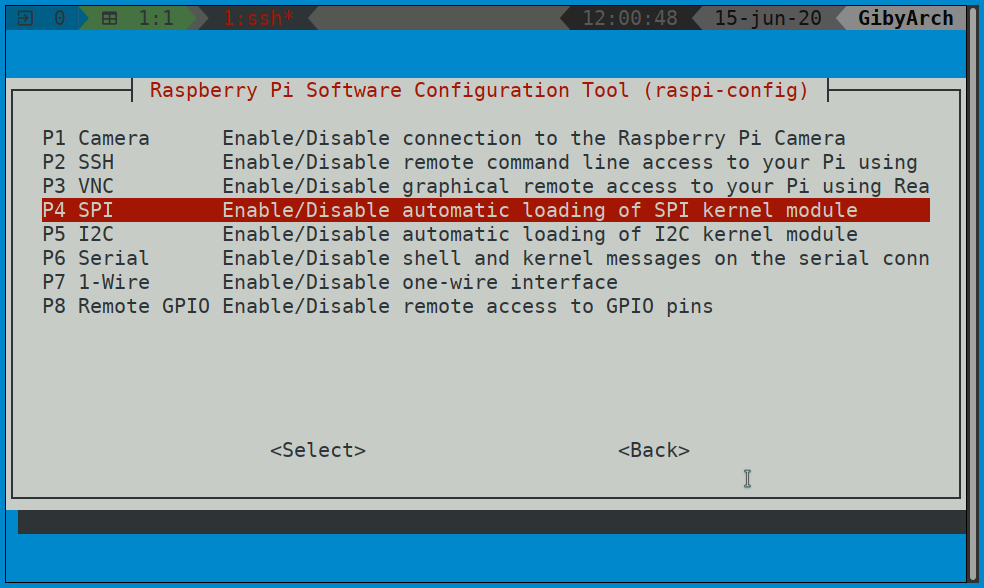
\includegraphics[width=.9\textwidth]{../pictures/SPI_raspi-config.png}
  \caption{SSH session to enable the SPI kernel module in Raspberry Pi using \cmd{raspi-config}. Inside \enquote{5 Interfacing options}}
  \label{fig:EnablingSPI}
\end{figure}

Then it would be necessary to install the GPIO access library from Raspberry repositories, so performing \cmd{sudo\, apt\, install\, wiringpi} the package manager should install \cmd{wiringpi} providing all necessary libraries.

After this, the reader will be in position to clone the controller from the github repository \cite{Dragino_DualChannelController_Rpi} and compile it performing the command shown in example \ref{ej:compiling_dual_channel_pkg} ---Like will be explained below, it is also important to note where \cmd{git} will clone the repository and where the reader will compile it, because the location of the \cmd{dual\_chan\_pkt\_fwd} binary is so critical for that systemd service (also included in the GitHub repository) \cmd{dual\_chan\_pkt\_fwd.service} works properly.
 
\begin{lstlisting}[%
  % float=ht,
  language=json,
  firstnumber=1,
  caption={Instructions to compile and install as a system service},
  label=ej:compiling_dual_channel_pkg
  ]
  cd ~
  git clone https://github.com/dragino/dual_chan_pkt_fwd
  cd dual_chan_pkt_fwd
  make
\end{lstlisting}

Once the controller is compiled, the reader must check the contents of \cmd{global\_conf.json}, for this projects, due to it is using the LoRa GPS HAT Single Channel LoRa \cite{DraginoRpiHat}, the pins configuration in \cmd{global\_conf.json} must be the following as stated by \cite{Dragino_DualChannelController_Rpi}

\begin{lstlisting}[%
  % float=ht,
  language=json,
  firstnumber=1,
  caption={defined pins in \cmd{global\_config.json}},
  label=ej:global_configJSON
  ]
  "pin_nss": 6,
  "pin_dio0": 7,
  "pin_rst": 0
\end{lstlisting}

I order to obtain the gateway ID the reader will need to perform the following command to run for the first time the \cmd{dual\_chan\_pkt\_fwd} binary, i.e. once the compilation process has produced the \cmd{dual\_chan\_pkt\_fwd} binary is necessary to run it directly to check the terminal output and find for the gateway ID.

\begin{lstlisting}[%
  % float=ht,
  language=json,
  firstnumber=1,
  caption={Running for the first time the LoRa HAT controller.},
  label=ej:Running_DualChann_Controller
  ]
  $ sudo ./dual_chan_pkt_fwd
  server: .address = router.eu.staging.thethings.network; .port = 1700; .enable = 1
  server: .address = router.eu.thethings.network; .port = 1700; .enable = 0
  Gateway Configuration
    your name (a@b.c)
    Dual channel pkt forwarder
    Latitude=0.00000000
    Longitude=0.00000000
    Altitude=10
    Interface: eth0
  Trying to detect module CE0 with NSS=6 DIO0=7 Reset=3 Led1=unused
  SX1276 detected on CE0, starting.
  Trying to detect module CE1 with NSS=6 DIO0=7 Reset=3 Led1=unused
  SX1276 detected on CE1, starting.
  Gateway ID: b8:27:eb:ff:ff:1b:14:9b
  Listening at SF7 on 868.100000 Mhz.
  Listening at SF7 on 868.100000 Mhz.
  -----------------------------------
  stat update: 2020-06-15 10:53:04 GMT no packet received yet 
\end{lstlisting}

So at the line 15 in the previous example \ref{ej:Running_DualChann_Controller}, the reader can see the Gateway ID, which wil be needed to connect this gateway to The Things Network stack. This ID is unique and it depends on the hardware.

After to have obtained the gateway ID (\cmd{b8:27:eb:ff:ff:1b:14:9b} for this Dragino HAT), the reader can proceed then to install the system service by perform \cmd{sudo make install}. As the content of \href{https://github.com/dragino/dual_chan_pkt_fwd/blob/master/Makefile#L22}{\cmd{Makefile}} shows at the line 22, \cmd{sudo make install} will copy the system service \cmd{dual\_chan\_pkt\_fwd.service} to the path \cmd{/lib/systemd/system/} and it will enable it in order to start the service ---the service will start the controller as the reader can see at line 9 in \href{https://github.com/dragino/dual_chan_pkt_fwd/blob/master/dual_chan_pkt_fwd.service#L9}{\cmd{dual\_chan\_pkt\_fwd.service}}--- at every system startup.\footnote{These kind of services are the way in which \cmd{systemd} manages the daemons running in background.} 

The reader must be aware of the path where is located the \cmd{dual\_chan\_pkt\_fwd} binary, this is so important because the service \cmd{dual\_chan\_pkt\_fwd.service} is using the absolute path to run the \cmd{dual\_chan\_pkt\_fwd} binary; So this could result in an error if the binary is not properly located or service is not properly modified.

Once the service is installed and all these point have been checked, the reader will be able to manage the service to

\begin{itemize}
  \item start it with \cmd{sudo systemctl start dual\_chan\_pkt\_fwd.service}
  \item stop it with \cmd{sudo systemctl stop dual\_chan\_pkt\_fwd.service}
  \item check its status with \cmd{systemctl status -l dual\_chan\_pkt\_fwd.service}
  \item check the journal with \cmd{journalctl -u dual\_chan\_pkt\_fwd.service}
\end{itemize}

These last two instructions show information about service status and \cmd{dual\_chan\_pkt\_fwd} status; in the picture \ref{fig:dual_chan_pkt_fwd-status} it can be seen the service active (running)

\begin{figure}[ht]
  \centering
  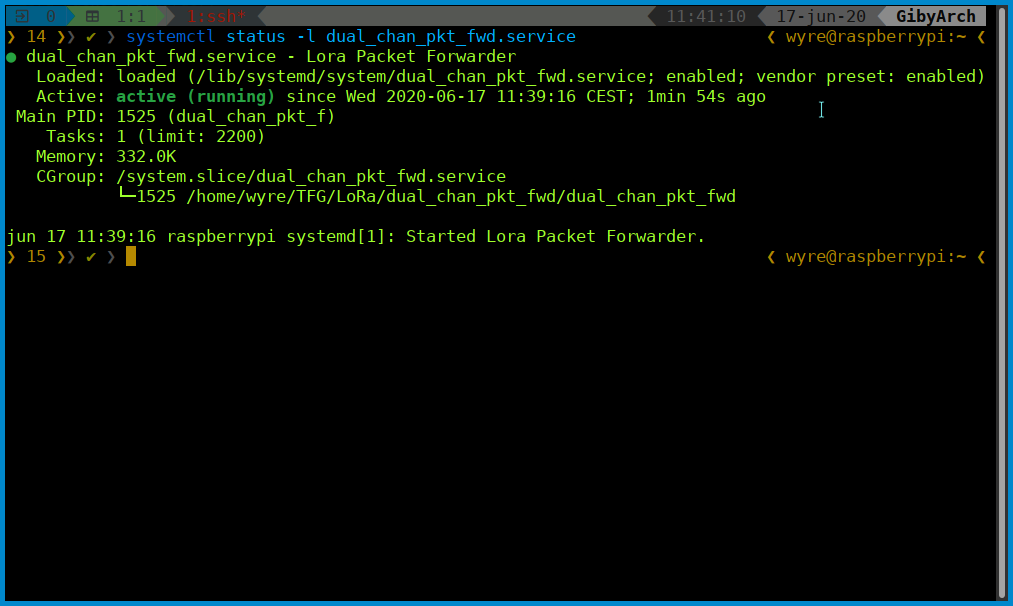
\includegraphics[width=.9\textwidth]{../pictures/pkt_fwd-service.png}
  \caption{systemd showing the \cmd{dual\_chan\_pkt\_fwd.service} status; it is active and running.}
  \label{fig:dual_chan_pkt_fwd-status}
\end{figure}

As it can be seen, this service was modified in order to reach properly the \cmd{dual\_chan\_pkt\_fwd} binary, which is not located in \cmd{/home/pi/dual\_chan\_pkt\_fwd/dual\_chan\_pkt\_fwd} (the default location defined for the binary in the \href{https://github.com/dragino/dual_chan_pkt_fwd/blob/master/dual_chan_pkt_fwd.service#L9}{GitHub repository}); mainly because the user is not called \cmd{pi} anymore but \cmd{wyre}, the path needs to be modified to that path containing the binary (\cmd{/home/wyre/TFG/LoRa/dual\_chan\_pkt\_fwd/dual\_chan\_pkt\_fwd})\footnote{This is a personal setup and is completely optional, the reader can choose their own path or even set up as suggested with \cmd{pi} user.}


After this the Raspberry Pi is ready to forward LoRa packets to the \href{https://github.com/dragino/dual_chan_pkt_fwd/blob/master/global_conf.json#L33}{specified server at line 33 in \cmd{global\_conf.json}}. Besides, the reader will be able to manage the Raspberry Pi through ssh service, so the Raspberry only precises any kind of internet access point and electrical power supply.

\subsection{Software}

The core of the software part is deployed using Docker containers \cite{Docker_container}. These docker containers are deploying essentially the following components

\begin{itemize}
  \item \textbf{IoTagent-LoRaWAN}, which is in charge of forward the traffic from TTN stack to Orion Context Broker.
  \item \textbf{Orion Context Broker}, this is the \myuline{core generic enabler}, in fact as indicated, this is the only one required component to the solution can be considered as \enquote{powered by FIWARE}. Besides this generic enabler requires a \textbf{Mongo database} to store entities and subscriptions among other things. 
  \item \textbf{QuantumLeap}, in order to make the context data persistent, this generic enabler is needed. Orion Context Broker works mainly with two elements; entities and subscriptions, however, for any created entity the context data does not persist in Mongo database, instead the context data will be replaced/updated; so creating a subscription which notifies to QuantumLeap, this generic enabler will store the context data in a \textbf{Crate database} to make it persistent. Also a \textbf{Redis database} is used for geocoding purposes, however this project will not deal with it ---this is why of this database is not even being included in the figure \ref{fig:GenView}.
  \item \textbf{Grafana}, this container is intended to provide a web interface to visualize and manage the retrieved context data. It stores its configuration and customization values in an embebed sqlite3 database; so there is not need for a separate container. 
\end{itemize}

These bold highlighted are the deployed containers that will be detailed later, many of them are not even part of FIWARE platform, though. First this document will expose how to set up the gateway, create an application and add devices inside The Things Network stack. 

\subsubsection{The Things Network Stack}\label{sssec:TTN_Stack}
This is a platform for the LoRaWAN protocol where is possible to manage gateways, devices and applications. It provides a centralized way to manage these kind of things regarding security too, generating several keys to tight the end-devices to the chosen server cloud solution (FIWARE in this case). There are three fundamental process the reader must follow to include nodes and gateways in the platform, those are luckily pretty well documented. 

\begin{itemize}
  \item \textbf{Register a gateway}; this is the process where \cmd{Gateway ID} shown in example \ref{ej:Running_DualChann_Controller} is needed; this process is, as indicated, well documented in \cite{Gateway_reg}.
  \item \textbf{Add an application}; this application will provide a set of security keys as well as a zone where manage different devices (these are basically the end-nodes i.e. the arduino microcontrollers). Is also documented in \cite{Add_application}.
  \item \textbf{Register a device} within added application; these devices will be ultimately the microcontrollers. Again the reader can find the relative documents in \cite{Device_reg}. 
\end{itemize}

Once these steps are completed, the TTN web interface will provide an overview with all data regarding the device like figure \ref{fig:dev_overview} shows. 

\begin{figure}[ht]
  \centering
  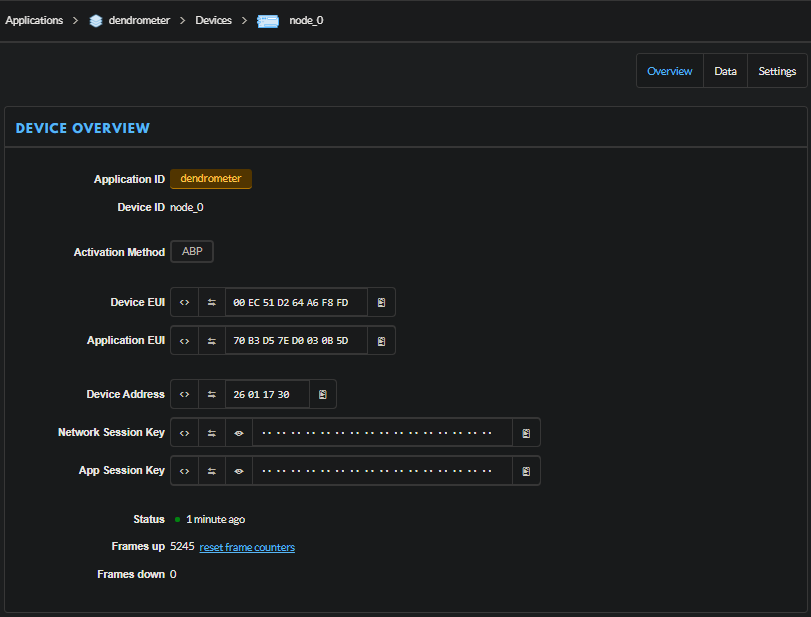
\includegraphics[width=.9\textwidth]{../pictures/TTN_dev_overview.png}
  \caption{A device overview.}
  \label{fig:dev_overview}
\end{figure}

Another important consideration inside TTN platform is to check which decoder is chosen for the received payloads, this can be checked by clicking on \cmd{Payload Formats} tab inside Application Overview. As it can be seen in figure \ref{fig:CayenneLPP_decoder}, it is so importan to choose the \cmd{CayenneLPP} decoder, because as indicated, \myuline{the payload is being encoded in the end-nodes using the CayenneLPP standard}. 

\begin{figure}[ht]
  \centering
  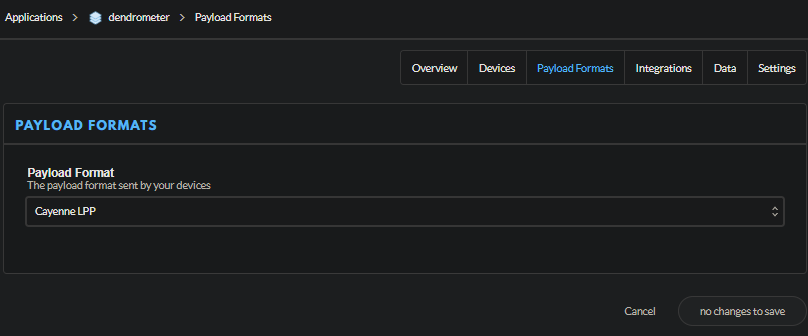
\includegraphics[width=.9\textwidth]{../pictures/TTN_Payload_Formats.png}
  \caption{Choosing CayenneLPP as payload decoder}
  \label{fig:CayenneLPP_decoder}
\end{figure}

Once this has been done, the microcontrollers has also been programmed and the gateway configured, the reader should be able to read the sensor data in the \cmd{Data} tab like figure \ref{fig:sens_data_TTN}

\begin{figure}[ht]
  \centering
  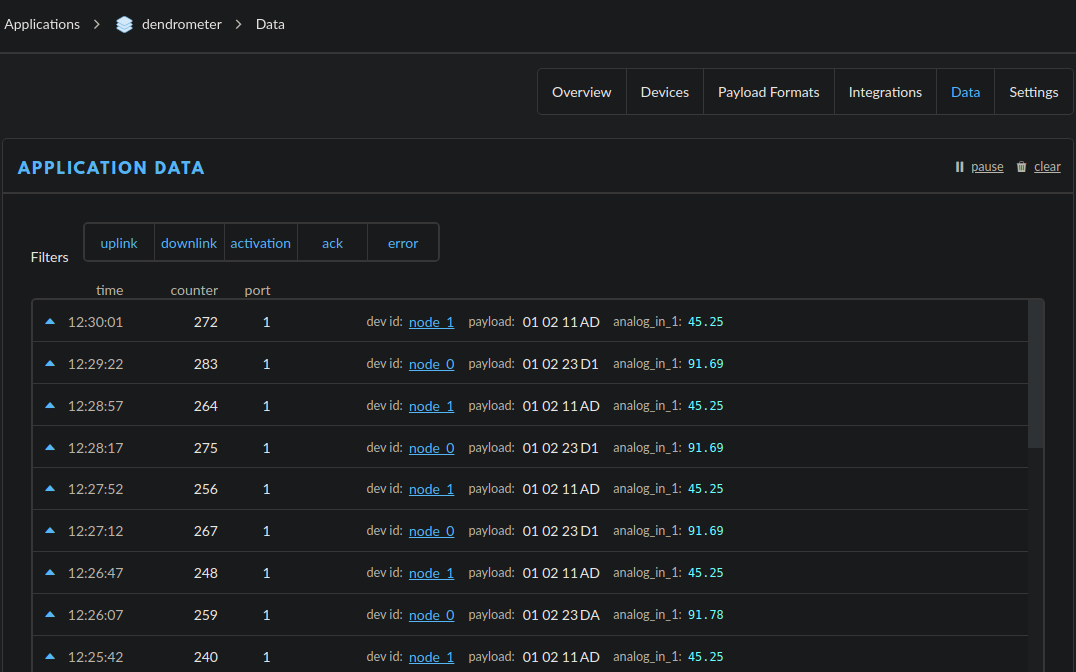
\includegraphics[width=.9\textwidth]{../pictures/TTN_sensors_data.png}
  \caption{Following sensors data in TTN.}
  \label{fig:sens_data_TTN}
\end{figure}

Then it should be possible to retrieve this data using the FIWARE IoTagent-LoRaWAN. The setup of this different FIWARE generic enablers will be explained in the next subsection, but essentially this IoTagent will use, as indicated previously, all those application and devices identifiers in order to manage the incoming context data from different microcontrollers (also called devices or end-nodes). 

\subsubsection{FIWARE}\label{sssec:FIWARE}
As shown in figure \ref{fig:GenView}, this solution is being implemented using particularly three FIWARE generic enablers, the most important one, of course, \textbf{Orion Context Broker}, also a LoRaWAN agent called \textbf{IoTagent-LoRaWAN} and finally to make data persistent, \textbf{QuantumLeap}.

The workflow is like picture \ref{fig:GenView} shows, first the IoTagent receives the context data from TTN, this IoTagent sends this context data to the Orion Context Broker and this latter notifies QuantumLeap the variations on the context data, thus QuantumLeap can proceed to store them into Crate database.

However this process does not happen out of the box, i.e. it is necessary to properly set up these generic enablers to get this workflow. This can be done following the FIWARE API documentation. These configuration can be donde using HTTP requests due to FIWARE essentially provides a RESTful API \cite{FIWARE_RESTful}, these HTTP requests can be performed using multiple clients like \cmd{curl} or \cmd{Postman} among others. This project in fact also provides a \href{https://github.com/WyRe/lora-arduino-dendrometer/tree/master/src/postman}{\cmd{Postman} collection and environment} that can be imported to manage them using a confortable graphical interface.

Anyway and after of this little introduction, the most important thing is to deploy all FIWARE generic enablers and its dependencies in a secure and stable way. This is why this project uses \cmd{docker} and \cmd{docker-compose} in order to ensure these modules deployment and execution. Again this project provides the \href{https://github.com/WyRe/lora-arduino-dendrometer/blob/master/src/fiware/docker-compose.yml}{\cmd{docker-compose.yml}} file to ensure a correct deployment. 

\begin{figure}[ht]
  \centering
  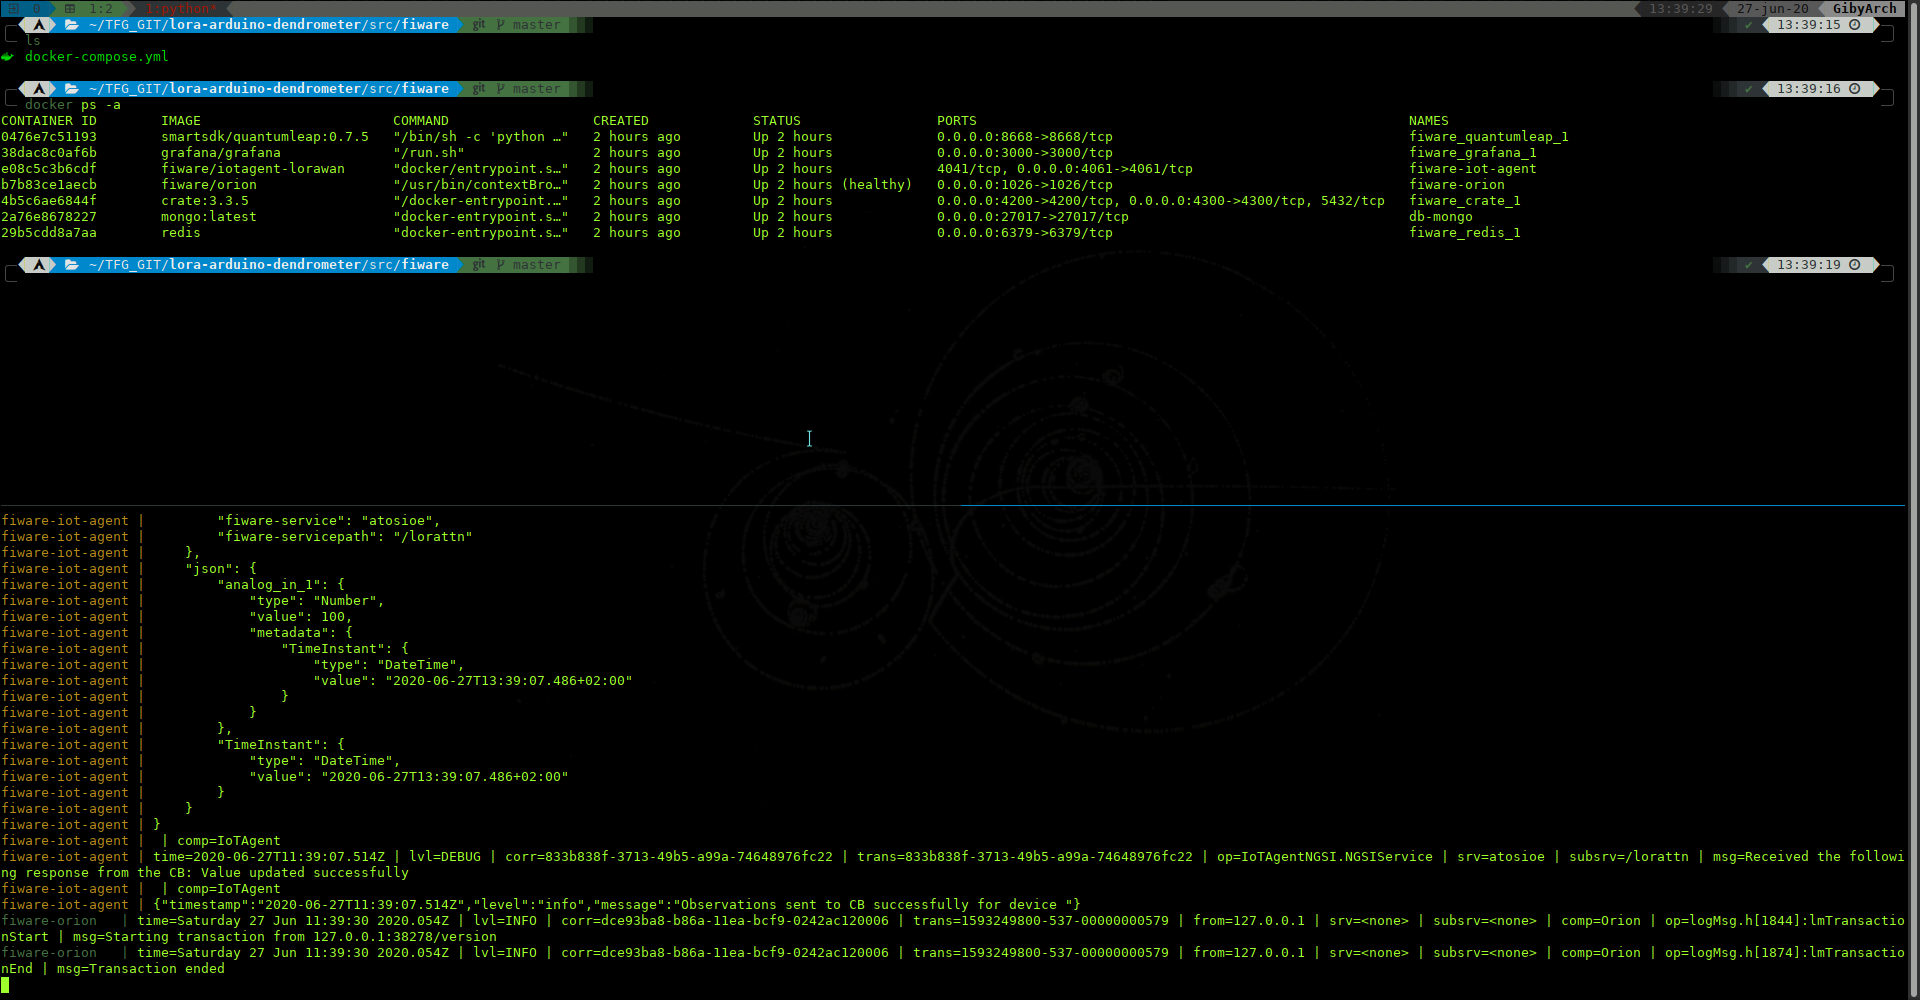
\includegraphics[width=.9\textwidth]{../pictures/docker_containers_deployed.png}  
  \caption{\cmd{tmux} showing docker containers status and logs.}
  \label{fig:docker_containers}
\end{figure}

So cloning the project and navigating to \cmd{src/fiware/} folder in the terminal the reader will must perform \cmd{docker-compose up -d} to deploy all containers and keep detached from the logs output. Once this has been done, performing \cmd{docker ps -a} will show the status of deployed containers, as figure \ref{fig:docker_containers} shows. In a similar way, to check the logs the reader could perform \cmd{docker-compose logs -f <NAME>} where the argument \cmd{<NAME>} is optional and when is not provided \cmd{docker-compose} will show logs for all containers; this is also shown in picture \ref{fig:docker_containers}.

When these containers are properly deployed, it should be possible to send the HTTP requests, however, these must follow a precise order; 


\begin{itemize}
  \item In a first place the reader will need to provision a new device for the \textbf{IoTagent-LoRaWAN}, this can be done performing a \cmd{POST} HTTP request whose body will include the necessary data to retrieve the TTN stack context data.
  
  \begin{lstlisting}[%
    % float=ht,
    language=json,
    firstnumber=1,
    caption={Device provisioning for IoTagent-LoRaWAN},
    label=ej:provisioning_devices
    ]
    $ curl localhost:4061/iot/devices -s -S -H 'Content-Type: application/json' -H 'Accept: application/json' -H 'fiware-service: atosioe' -H 'fiware-servicepath: /lorattn' -d @- <<EOF
    {
      "devices": [
        {
          "device_id": "node_0",
          "entity_name": "LORA-N-0",
          "entity_type": "LoraDevice",
          "timezone": "Europe/Madrid",
          "attributes": [
            {
              "object_id": "analog_in_1",
              "name": "analog_in_1",
              "type": "Number"
            }
          ],
          "internal_attributes": {
            "lorawan": {
              "application_server": {
                "host": "eu.thethings.network",
                "username": "dendrometer",
                "password": "ttn-account-v2.173lH8wwDiIRC8E2JgM9ScXyuNRlPpMefpazS0TIhnU",
                "provider": "TTN"
              },
              "dev_eui": "00EC51D264A6F8FD",
              "app_eui": "70B3D57ED0030B5D",
              "application_id": "dendrometer",
              "application_key": "3736B21218C4443F639FAF4114B723A1",
              "data_model": "cayennelpp"
            }
          }
        }
      ]
    }
    EOF
  \end{lstlisting}

  As example \ref{ej:provisioning_devices} shows, is mandatory to provide a \cmd{"device\_id"}, which would be desirable to match with de TTN device ID, an \cmd{"entity\_name"} in order to make Orion Context Broker create that entity and also an \cmd{"username"} and \cmd{"application\_id"} that must match with the application ID in TTN. Besides It will be needed the \cmd{"password"}, which can be obtained from the Application Overview in TTN website and the \cmd{"dev\_eui"}, \cmd{"app\_eui"} and \cmd{"application\_key"}, all of these ---relative to the created device--- are available into TTN dashboard. This \cmd{POST} request is included in the \cmd{Postman} collection provided by this project repository; of course \myuline{the reader will need to replace the keys in the environment for their own}. 

  When a new device is created, \textbf{IoTagent-LoRaWAN} causes that \textbf{Orion Context Broker} creates a new entity. In fact this can be checked by performing a \cmd{GET} HTTP request, 

  \begin{lstlisting}[%
    % float=ht,
    language=json,
    firstnumber=1,
    caption={Querying OrionCB for entities list.},
    label=ej:OrionCB_entities_Get
    ]
    $ curl localhost:1026/v2/entities \                                                                       
       -H 'fiware-service: atosioe' \
       -H 'fiware-servicepath: /lorattn' | python -mjson.tool
      % Total    % Received % Xferd  Average Speed   Time    Time     Time  Current
                                     Dload  Upload   Total   Spent    Left  Speed
    100   248  100   248    0     0   4275      0 --:--:-- --:--:-- --:--:--  4275
    [
        {
            "id": "LORA-N-0",
            "type": "LoraDevice",
            "TimeInstant": {
                "type": "DateTime",
                "value": "2020-06-27T15:58:48.00Z",
                "metadata": {}
            },
            "analog_in_1": {
                "type": "Number",
                "value": 55.03,
                "metadata": {
                    "TimeInstant": {
                        "type": "DateTime",
                        "value": "2020-06-27T15:58:48.00Z"
                    }
                }
            }
        }
    ]
  \end{lstlisting}

  Example \ref{ej:OrionCB_entities_Get} shows the response of that \cmd{GET} request when a new entity is created by Orion Context Broker.

  \item Secondly, after have created the device and therefore the entity, the next thing to do is to create a subscription in order to Orion Context Broker notifies somewhere ---QuantumLeap in this case. In a similar way, to create this subscription the reader can perform a \cmd{POST} request against Orion Context Broker, so as example \ref{ej:OrionCB_subscription} shows, 
  
  \begin{lstlisting}[%
    % float=ht,
    language=json,
    firstnumber=1,
    caption={Creating a subscription to notify QuantumLeap.},
    label=ej:OrionCB_subscription
    ]
    $ curl localhost:1026/v2/subscriptions -s -S -H 'Content-Type: application/json' -H 'fiware-service: atosioe' -H 'fiware-servicepath: /lorattn' -d @- <<EOF
    {
      "description": "A subscription to get info about LORA-N-0",
      "subject": {
        "entities": [
          {
            "id": "LORA-N-0",
            "type": "LoraDevice"
          }
        ],
        "condition": {
          "attrs": [
            "analog_in_1"
          ]
        }
      },
      "notification": {
        "http": {
          "url": "http://quantumleap:8668/v2/notify"
        },
        "attrs": [
          "analog_in_1"
        ],
        "metadata": ["dateCreated", "dateModified"]
      },
      "throttling": 5
    }
    EOF
  \end{lstlisting}

  As the reader can see, for this subscription has been set up the \cmd{"url": "http://quantumleap:8668/v2/notify"} i.e. QuantumLeap will be notified at any change in the entity with \cmd{"id": "LORA-N-0"}; also it's a good practice to check that all went as expected, so sending a \cmd{GET} request the response should be like example \ref{ej:OrionCB_subscriptions_get} 

  \begin{lstlisting}[%
    % float=ht,
    language=json,
    firstnumber=1,
    caption={Querying for all existent subscriptions in OrionCB.},
    label=ej:OrionCB_subscriptions_get
    ]
    $ curl localhost:1026/v2/subscriptions \
    -H 'fiware-service: atosioe' \
    -H 'fiware-servicepath: /lorattn' | python -mjson.tool
      % Total    % Received % Xferd  Average Speed   Time    Time     Time  Current
                                     Dload  Upload   Total   Spent    Left  Speed
    100   535  100   535    0     0   9067      0 --:--:-- --:--:-- --:--:--  9067
    [
        {
            "id": "5ef772be8153f85ef485b5fd",
            "description": "A subscription to get info about LORA-N-0",
            "status": "active",
            "subject": {
                "entities": [
                    {
                        "id": "LORA-N-0",
                        "type": "LoraDevice"
                    }
                ],
                "condition": {
                    "attrs": [
                        "analog_in_1"
                    ]
                }
            },
            "notification": {
                "timesSent": 17,
                "lastNotification": "2020-06-27T16:40:56.00Z",
                "attrs": [
                    "analog_in_1"
                ],
                "onlyChangedAttrs": false,
                "attrsFormat": "normalized",
                "http": {
                    "url": "http://quantumleap:8668/v2/notify"
                },
                "metadata": [
                    "dateCreated",
                    "dateModified"
                ],
                "lastSuccess": "2020-06-27T16:40:56.00Z",
                "lastSuccessCode": 200
            },
            "throttling": 5
        }
    ]

  \end{lstlisting}

\end{itemize}

Once these two steps have been performed successfully, the context data should be routed to the Crate database where will be persistent. 

\subsubsection{Grafana}\label{sssec:Grafana}
Grafana is a powerful dashboard used at many scenarios in the software industry, it allows to monitor almost everything the reader can imagine; due to it is actually capable to acquire the data from multiple sources. In this project will be used in order to monitor the context data along the time.

This web application can be accessed via \cmd{http://localhost:3000} in the web browser ---the file \cmd{docker-compose.yml} is already setup to expose that port and allow the user to connect Grafana in that way. The default credentials for the first access are \cmd{username: admin} and \cmd{password: admin}. Once the reader has accessed for a first time is possible to modify those credentials or even create new users with different privileges.

\begin{figure}[ht]
  \centering
  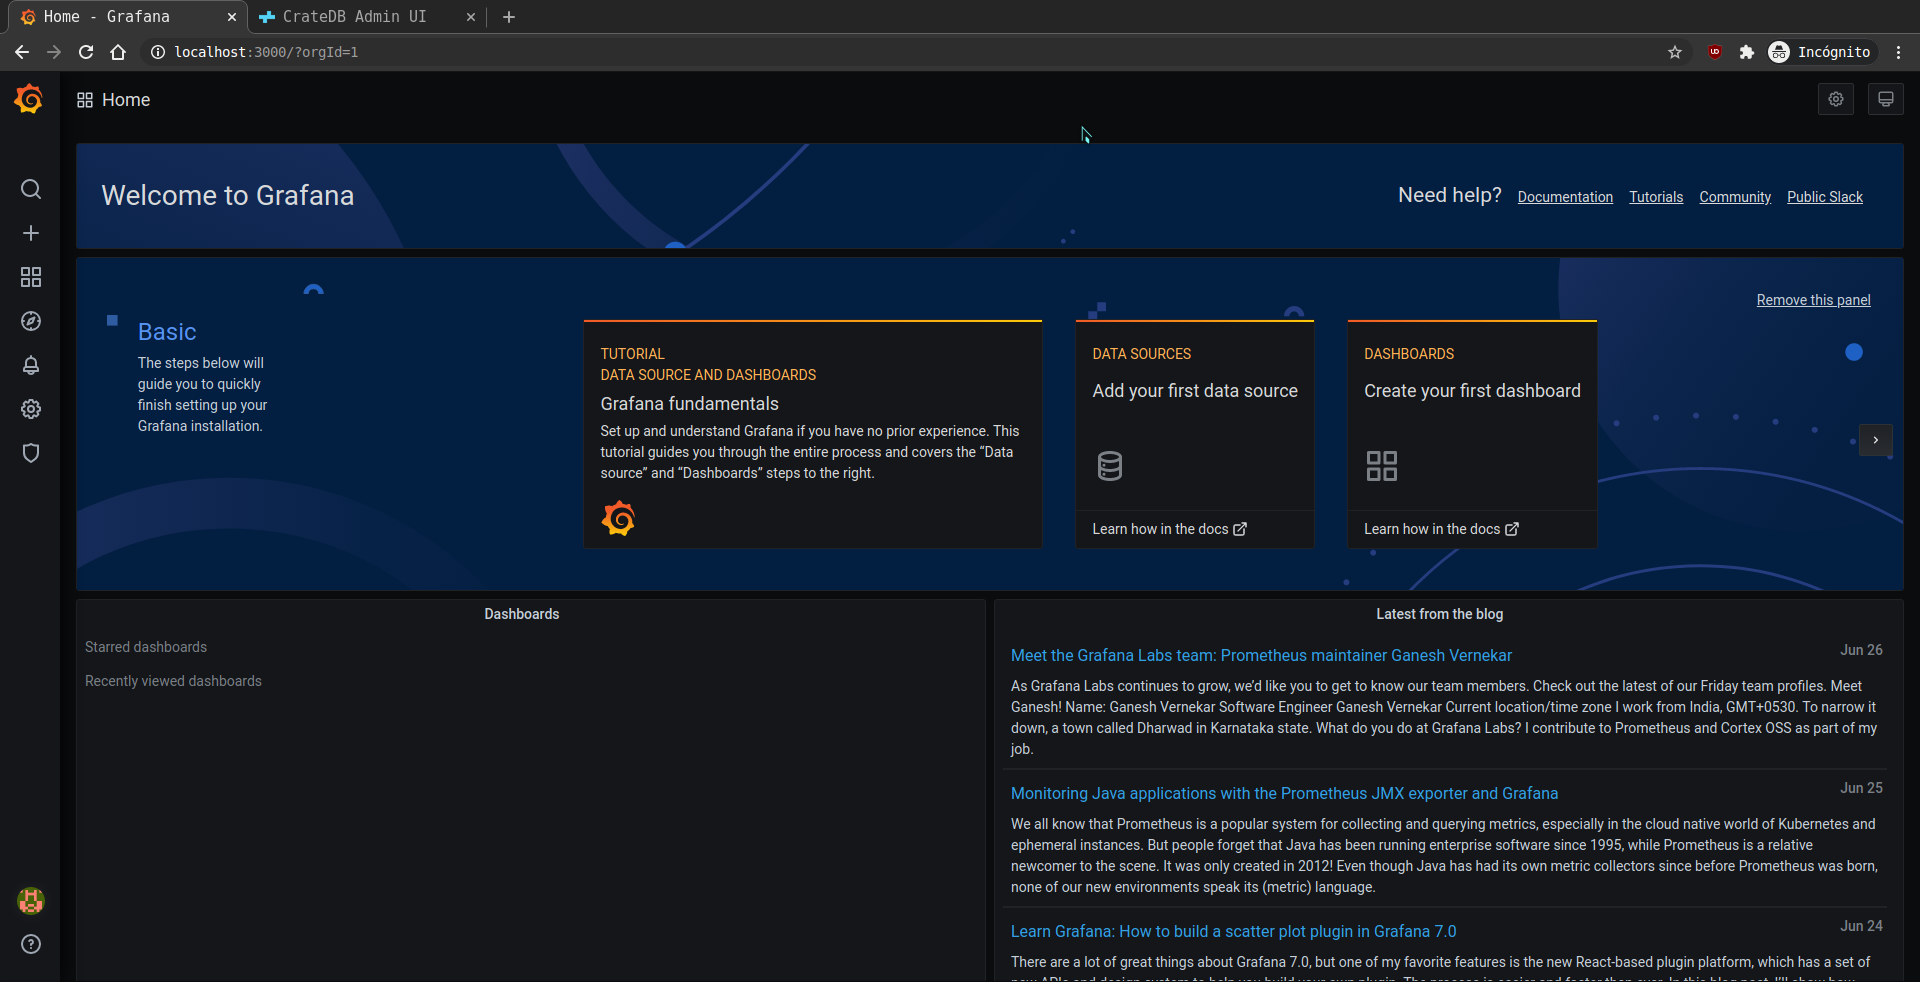
\includegraphics[width=.9\textwidth]{../pictures/Grafana_home.png}
  \caption{Grafana home view.}
  \label{fig:grafana_home}
\end{figure}

AS the central panel in the home view indicates, there are two fundamental task that must be performed to get a detailed view of our context data; these are to add a data source and set up a new dashboard. 

To add a new data source the reader can use the left sidebar or click where says \enquote{Add your first dada source} in the home view. CrateDB is PostgreSQL compatible, so it must be chosen a PostgreSQL database and fill the form with the data shown in figure \ref{fig:Grafana_add_datasource}

\begin{figure}[ht]
  \centering
  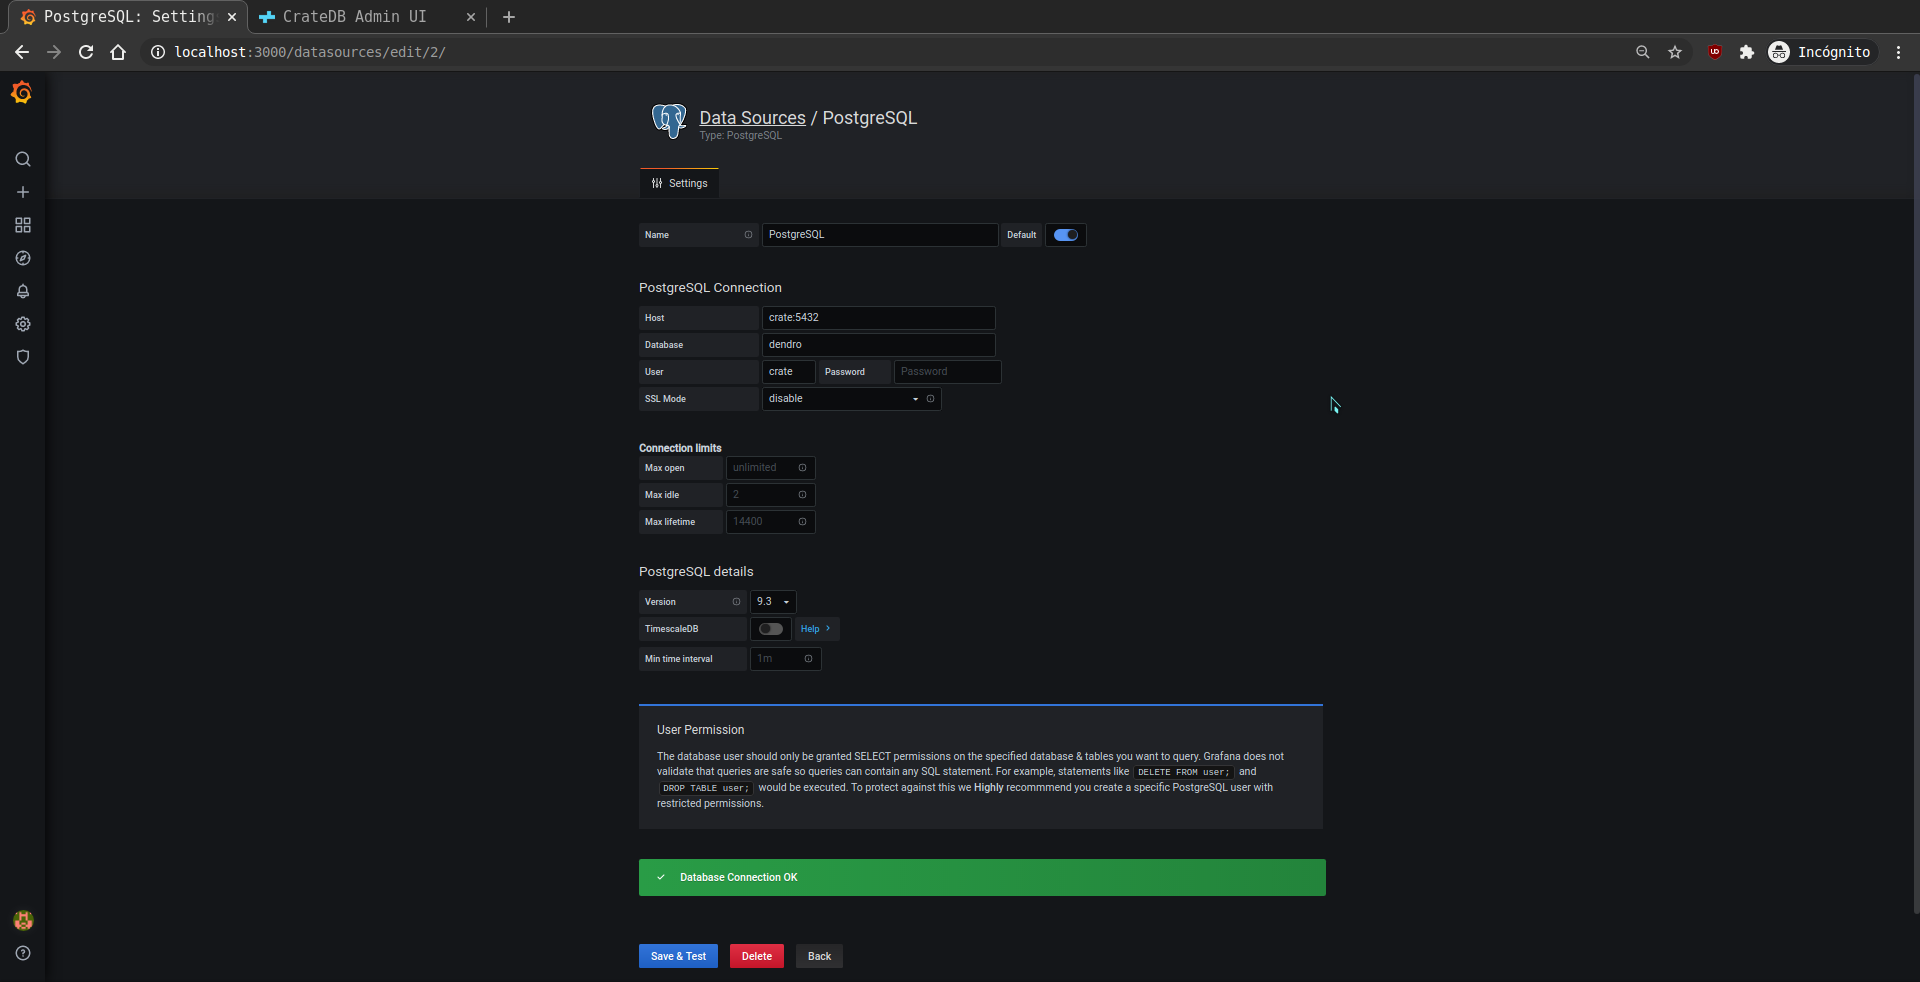
\includegraphics[width=.9\textwidth]{../pictures/Grafana_add_datasource.png}
  \caption{Adding CrateDB as the data source}
  \label{fig:Grafana_add_datasource}
\end{figure}

\enquote{Host} must be \cmd{crate:5432} because is the port which grafana uses to queries under postgres protocol, this can be seen also in figure \ref{fig:docker_containers} another important credential is the \enquote{User} that must be \cmd{crate} with no password because CrateDB does not set anyone by default, \enquote{Database} can be set arbitrarily, and finally the \enquote{SSL} has to be disabled. 

\begin{figure}[ht]
  \centering
  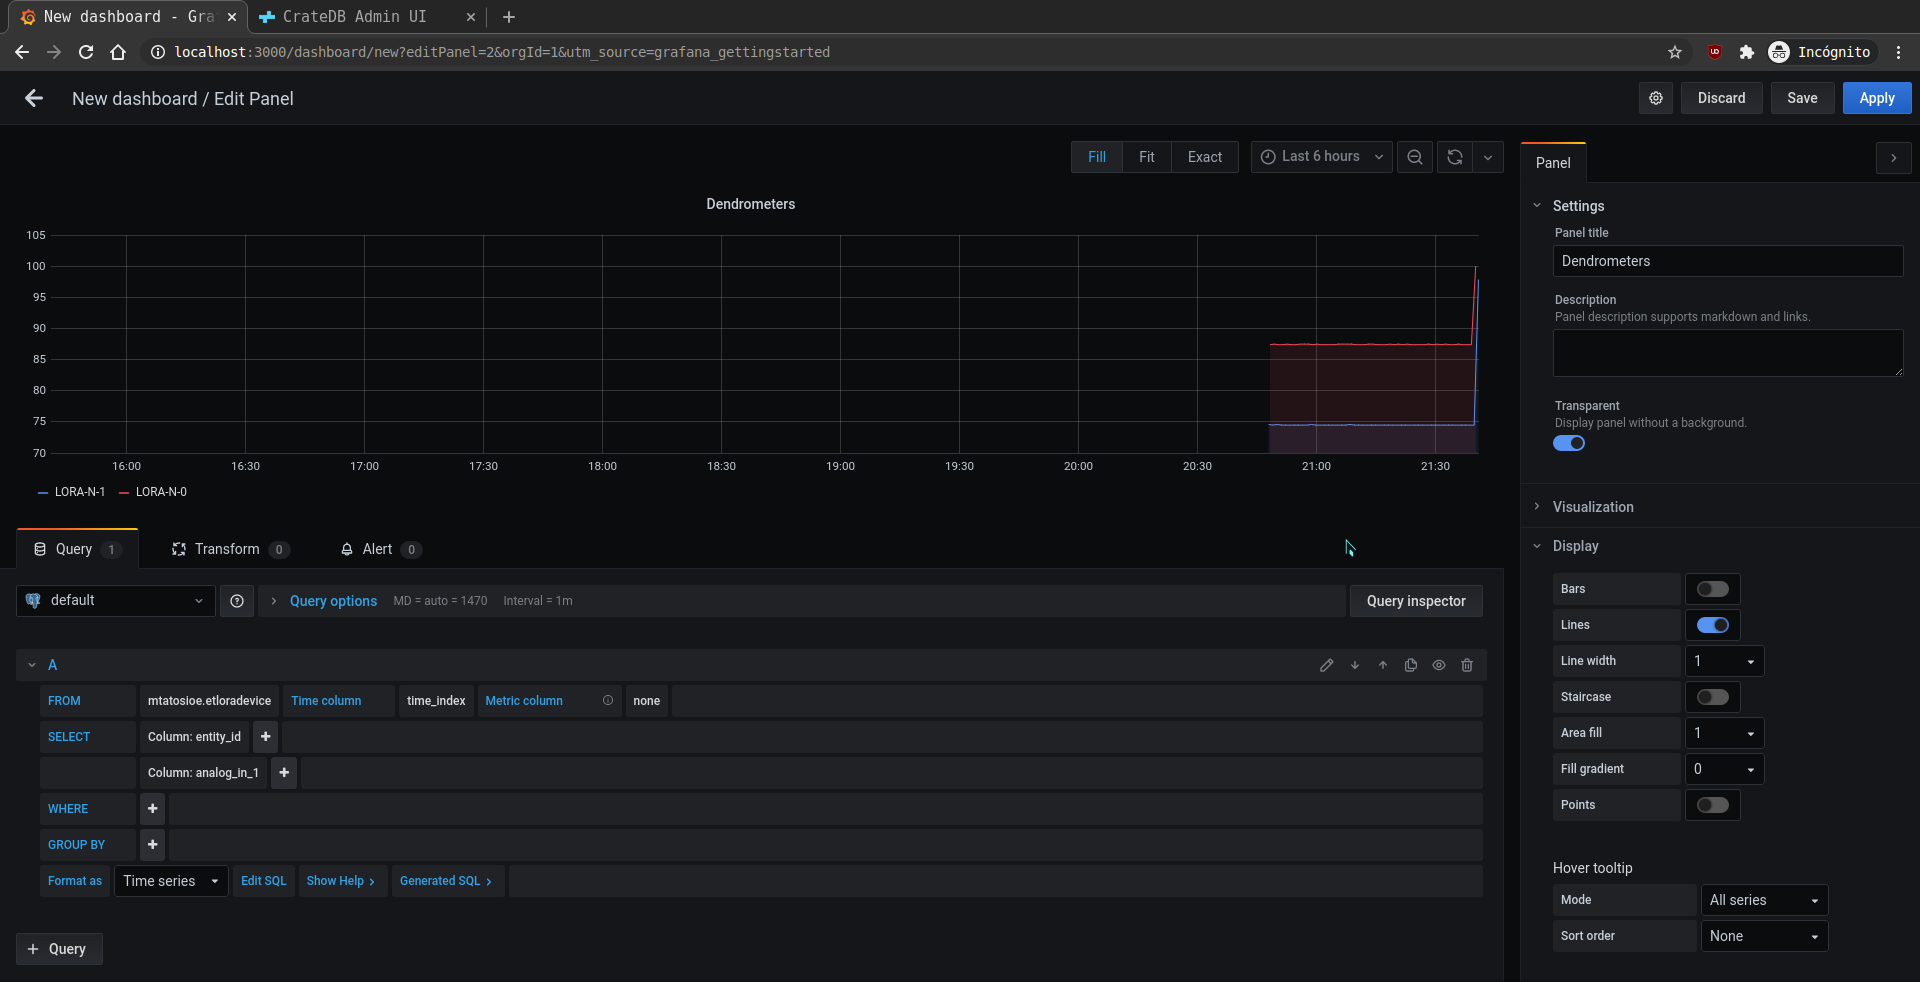
\includegraphics[width=.9\textwidth]{../pictures/Grafana_panel_setup.png}
  \caption{Setting up a panel.}
  \label{fig:panel_setup}
\end{figure}

To get the panel drawing the CrateDB stored context data, the reader must specify a query to retrieve the data from the database. This can be done in the \enquote{Query} tab below the graph shown in picture \ref{fig:panel_setup}, here the user could use the graphical interface or write the query manually by clicking on the pencil button at the right, so essentially the query should looks as follows in example \ref{ej:CrateDB_query}

\begin{lstlisting}[%
  % float=ht,
  language=json,
  firstnumber=1,
  caption={Query to retrieve the stored context data.},
  label=ej:CrateDB_query
  ]
    SELECT
    time_index AS "time",
    entity_id,
    analog_in_1
  FROM mtatosioe.etloradevice
  ORDER BY 1
\end{lstlisting}

The table name \cmd{mtatosioe.etloradevice} can be found inside CrateDB admin panel, which can be accessed in \cmd{http://localhost:4200/\#!/tables} from the web browser. So after clicking on \enquote{Apply} button on top right corner the reader should have something similar to figure \ref{fig:final_panel}

\begin{figure}[ht]
  \centering
  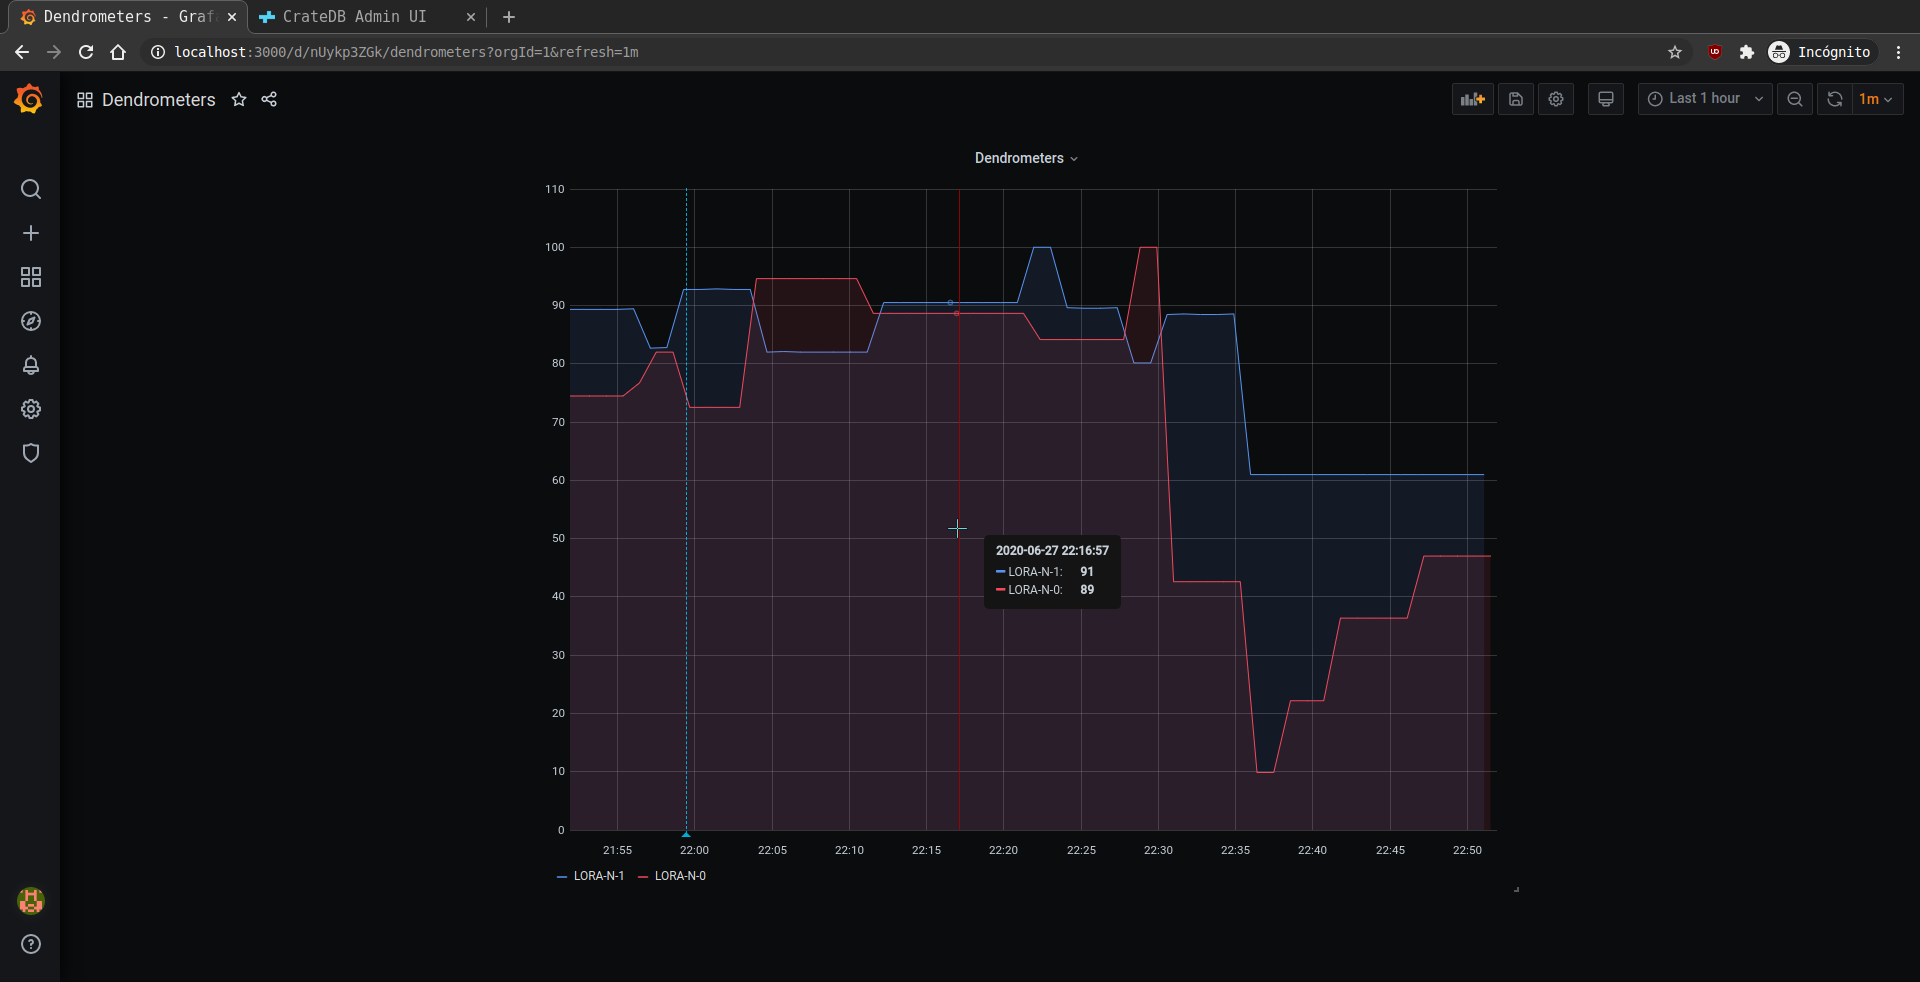
\includegraphics[width=.9\textwidth]{../pictures/Grafana_final_panel.png}
  \caption{Dendrometers panel}
  \label{fig:final_panel}
\end{figure}

Grafana has a wide set of options intended to monitor different kind of systems, it can represent data in different type of graphics and even allows export to csv format, this can be useful for a more deep analysis using other technologies like, for instance, R, a well-known language widely used for statistical analysis.

Of course, this context data could be acquired directly from CrateDB by means of some custom application developed specifically to this task, however this is beyond of the purpose of this project. Maybe in a future a feature like this could be implemented. 

\subsubsection{FIWARE API Graphical User Interface}\label{sssec:API_GUI}
Finally, to make more friendly the FIWARE interaction exposed in \hyperref[sssec:FIWARE]{FIWARE} subsection, this project also provide a simple and light \href{https://github.com/WyRe/lora-arduino-dendrometer/blob/master/src/api-gui/api-gui.py}{graphical user interface}. This graphical interface has been developed using the well-known tkinter library in python, it requires also a few python modules that are specified in \href{https://github.com/WyRe/lora-arduino-dendrometer/blob/master/src/api-gui/pip_requirements.txt}{\cmd{/src/api-gui/pip\_requirements.txt}}, in fact the user should be able to install them by performing in a terminal the following command \cmd{pip install -r pip\_requirements.txt}.

When the requirements are satisfied and all docker containers are running properly\footnote{In a first place the GUI will retrieve the versions for Orion Context Broker, IoTagent-LoRaWAN and QuantumLeap, so if they are not running the GUI wont open.} the GUI can be run performing \cmd{./api-gui.py}; this should open the window shown by figure \ref{fig:GUI_app_keys}

\begin{figure}[ht]
  \centering
  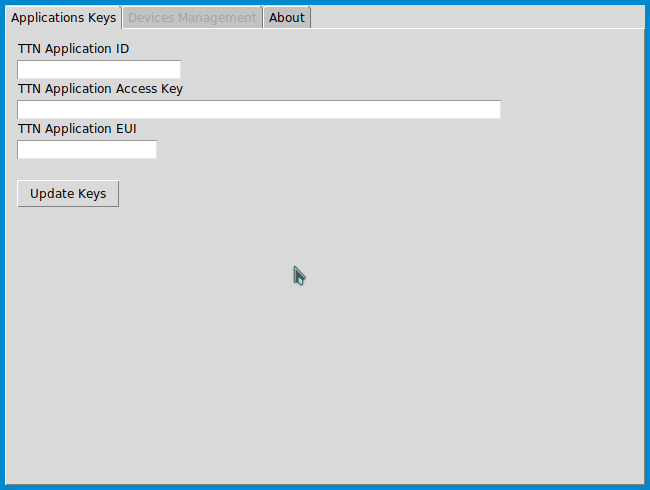
\includegraphics[width=.9\textwidth]{../pictures/GUI_app_keys.png}
  \caption{First view of \cmd{api-gui.py}}
  \label{fig:GUI_app_keys}
\end{figure}

To check Orion Context Broker, IoTagent-LoRaWAN and QuantumLeap versions running in the docker containers the reader has to click on \enquote{About} tab, however, this first shown tab ---\enquote{Application Keys}--- is the most important one because without complete all the required info won't be enabled the \enquote{Devices Management} tab. Actually this tab performs a series of checks regarding TTN keys. Following the same TTN requirements, 

\begin{itemize}
  \item TTN Application ID must be greater than 2 characters.
  \item TTN Application Access Key must starts with \cmd{ttn-account} string.
  \item TTN Application EUI must be 16 characters long and be hexadecimal. 
\end{itemize}
When any of this requirements are not fulfilled the related label will turn red as figure \ref{fig:GUI_app_keys_fail} shows

\begin{figure}[ht]
  \centering
  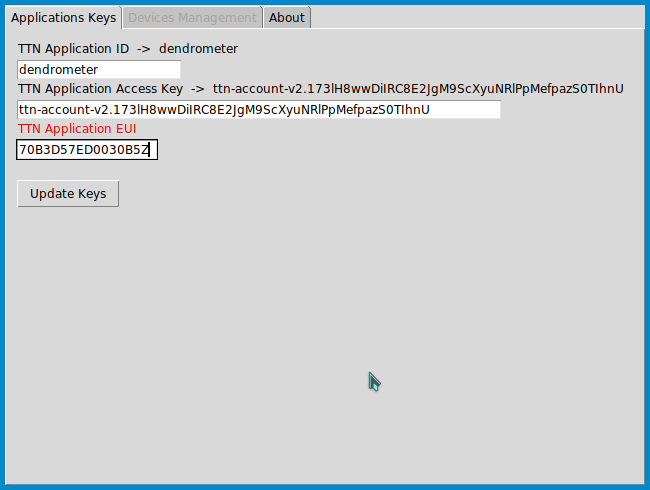
\includegraphics[width=.9\textwidth]{../pictures/GUI_app_keys_fail.png}
  \caption{TTN Application EUI must be hexadecimal} 
  \label{fig:GUI_app_keys_fail}
\end{figure}

This information of course must match exactly with information provided by TTN, actually the \enquote{TTN Application Acess Key} and \enquote{TTN Application EUI} are provided by TTN, however the \enquote{TTN Application ID} must be chosen by the user when a new application is created using the TTN web interface, but this ID must be unique and it must be at least 3 characters long, that is why the developed GUI follows the same criteria.

When the keys are updated properly the labels over the text fields are also updated with the chosen values and the \enquote{Devices Management} tab is enabled. This tab provides also a more friendly interface to manage devices. In a similar way this info will must match with the info provided by TTN interface, so that as figure \ref{fig:device_management_tab}

\begin{figure}[ht]
  \centering
  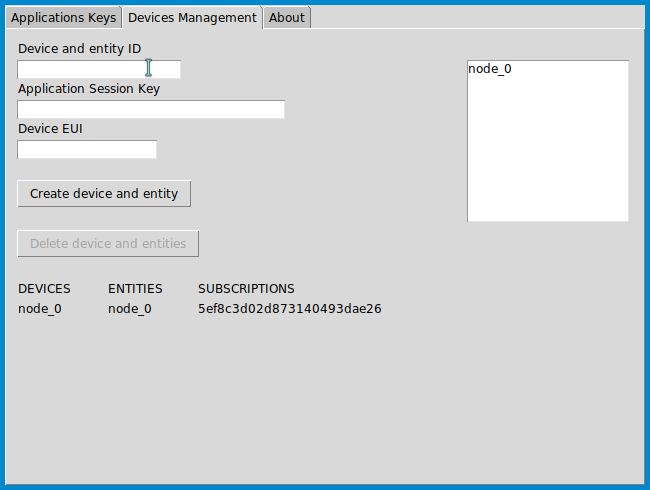
\includegraphics[width=.9\textwidth]{../pictures/GUI_device_management.png}
  \caption{Device Management tab}
  \label{fig:device_management_tab}
\end{figure}

This view allows the user to create and delete devices ---along with its entities and subscriptions--- nevertheless, the \enquote{Delete device and entities} button remains disabled until a device is chosen in the right list. In a similar way than \enquote{Applications Keys}, to add a new device to FIWARE deployed instance by docker, all keys must fullfil a set of minimum requirements; as it can be seen in picture \ref{fig:adding_dev}

\begin{itemize}
  \item Device entity and ID must be also unique and it has to be at least 3 characters long. Moreover, this ID must match exactly with the ID chosen in TTN interface when the device is created,
  \item Application Session Key must be 32 characters long and also an hexadecimal string.
  \item Device EUI has to be 16 characters long and again an hexadecimal string.
\end{itemize}

These keys can be obtained from TTN as it can be seen in screenshot \ref{fig:dev_overview} ---this screenshot shows info about \cmd{node\_0}, though. We can see in picture \ref{fig:adding_dev}, that there was a problem with \enquote{Device EUI}, this was caused because of the final \cmd{Z} letter in the string which doesn't belong to hexadecimal characters set.

\begin{figure}[htp]
  \centering
  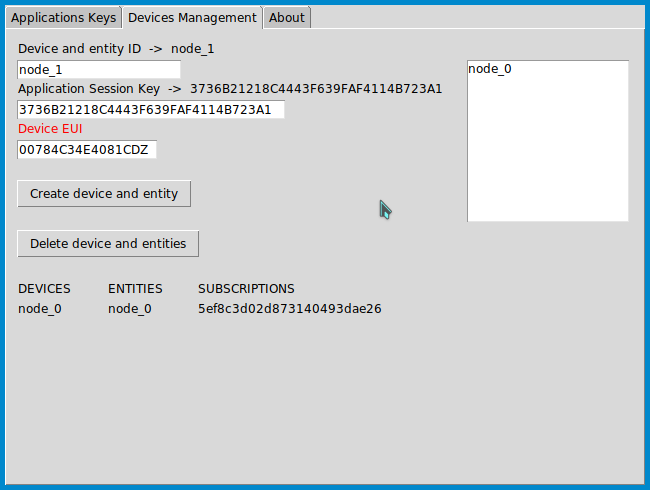
\includegraphics[width=.9\textwidth]{../pictures/GUI_add_device.png}
  \caption{Trying to add a new device}
  \label{fig:adding_dev}
\end{figure}

\begin{figure}[htp]
  \centering
  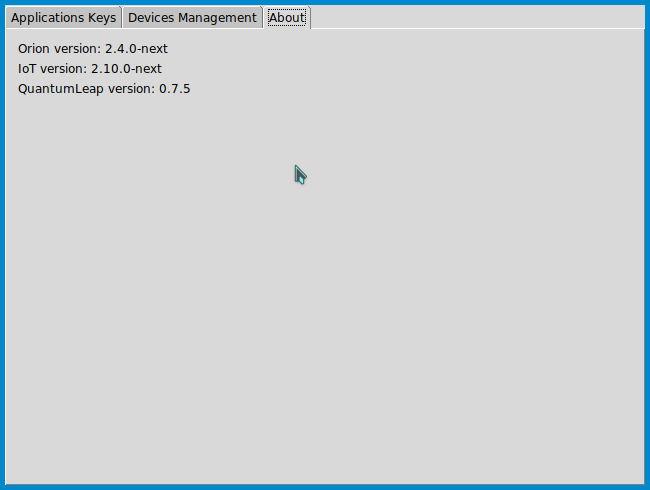
\includegraphics[width=.9\textwidth]{../pictures/GUI_about_tab.png}
  \caption{Running versions in About tab.}
  \label{fig:about_tab}
\end{figure}

Finally, as indicated, the \enquote{About} tab shows the versions info as it can be seen in \ref{fig:about_tab}. The QuantumLeap version is specified in \cmd{docker-compose.yml} file as well as the CrateDB version, this is to ensure compatibility between QuantumLeap and CrateDB; however, Orion Context Broker and IoTagent-LoRaWAN versions are not specified so they should be always the latests, this is why could be helpful to retrieve these. 

\begin{figure}[ht]
  \centering
  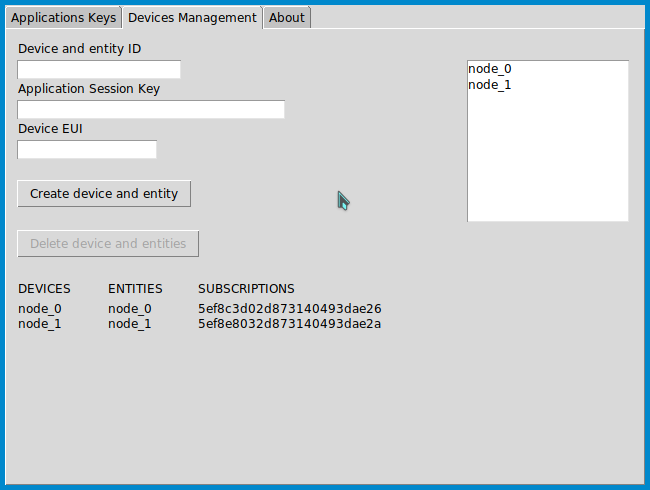
\includegraphics[width=.9\textwidth]{../pictures/GUI_device_management_2nodes.png}
  \caption{Graphical interface showing 2 created nodes}
  \label{fig:GUI_2nodes}
\end{figure}

As figure \ref{fig:GUI_2nodes} shows, once a node is created is added to the list, subscription and entity ID are useful to remove manually just a subscription or an entity by performing a manual \cmd{DELETE} request, in fact have been also included several \cmd{DELETE} requests in the attached Postman collection, however, when a node is deleted using this graphical interface button is also being removed its entity and its subscription.

\clearpage{\pagestyle{empty}\cleardoublepage}\thispagestyle{plain}  % Forces the next section to start in an odd page.
\section{Proof of concept, deployment}
Due to circumstances at early 2020, this section has been reduced, instead of test the system in a real production environment, this section will focus on summarize needed steps/stages to deploy the system properly. Although these steps are already detailed separately, this section tries to put them together to give a consistent and practical point of view.

\begin{figure}[ht]
  \centering
  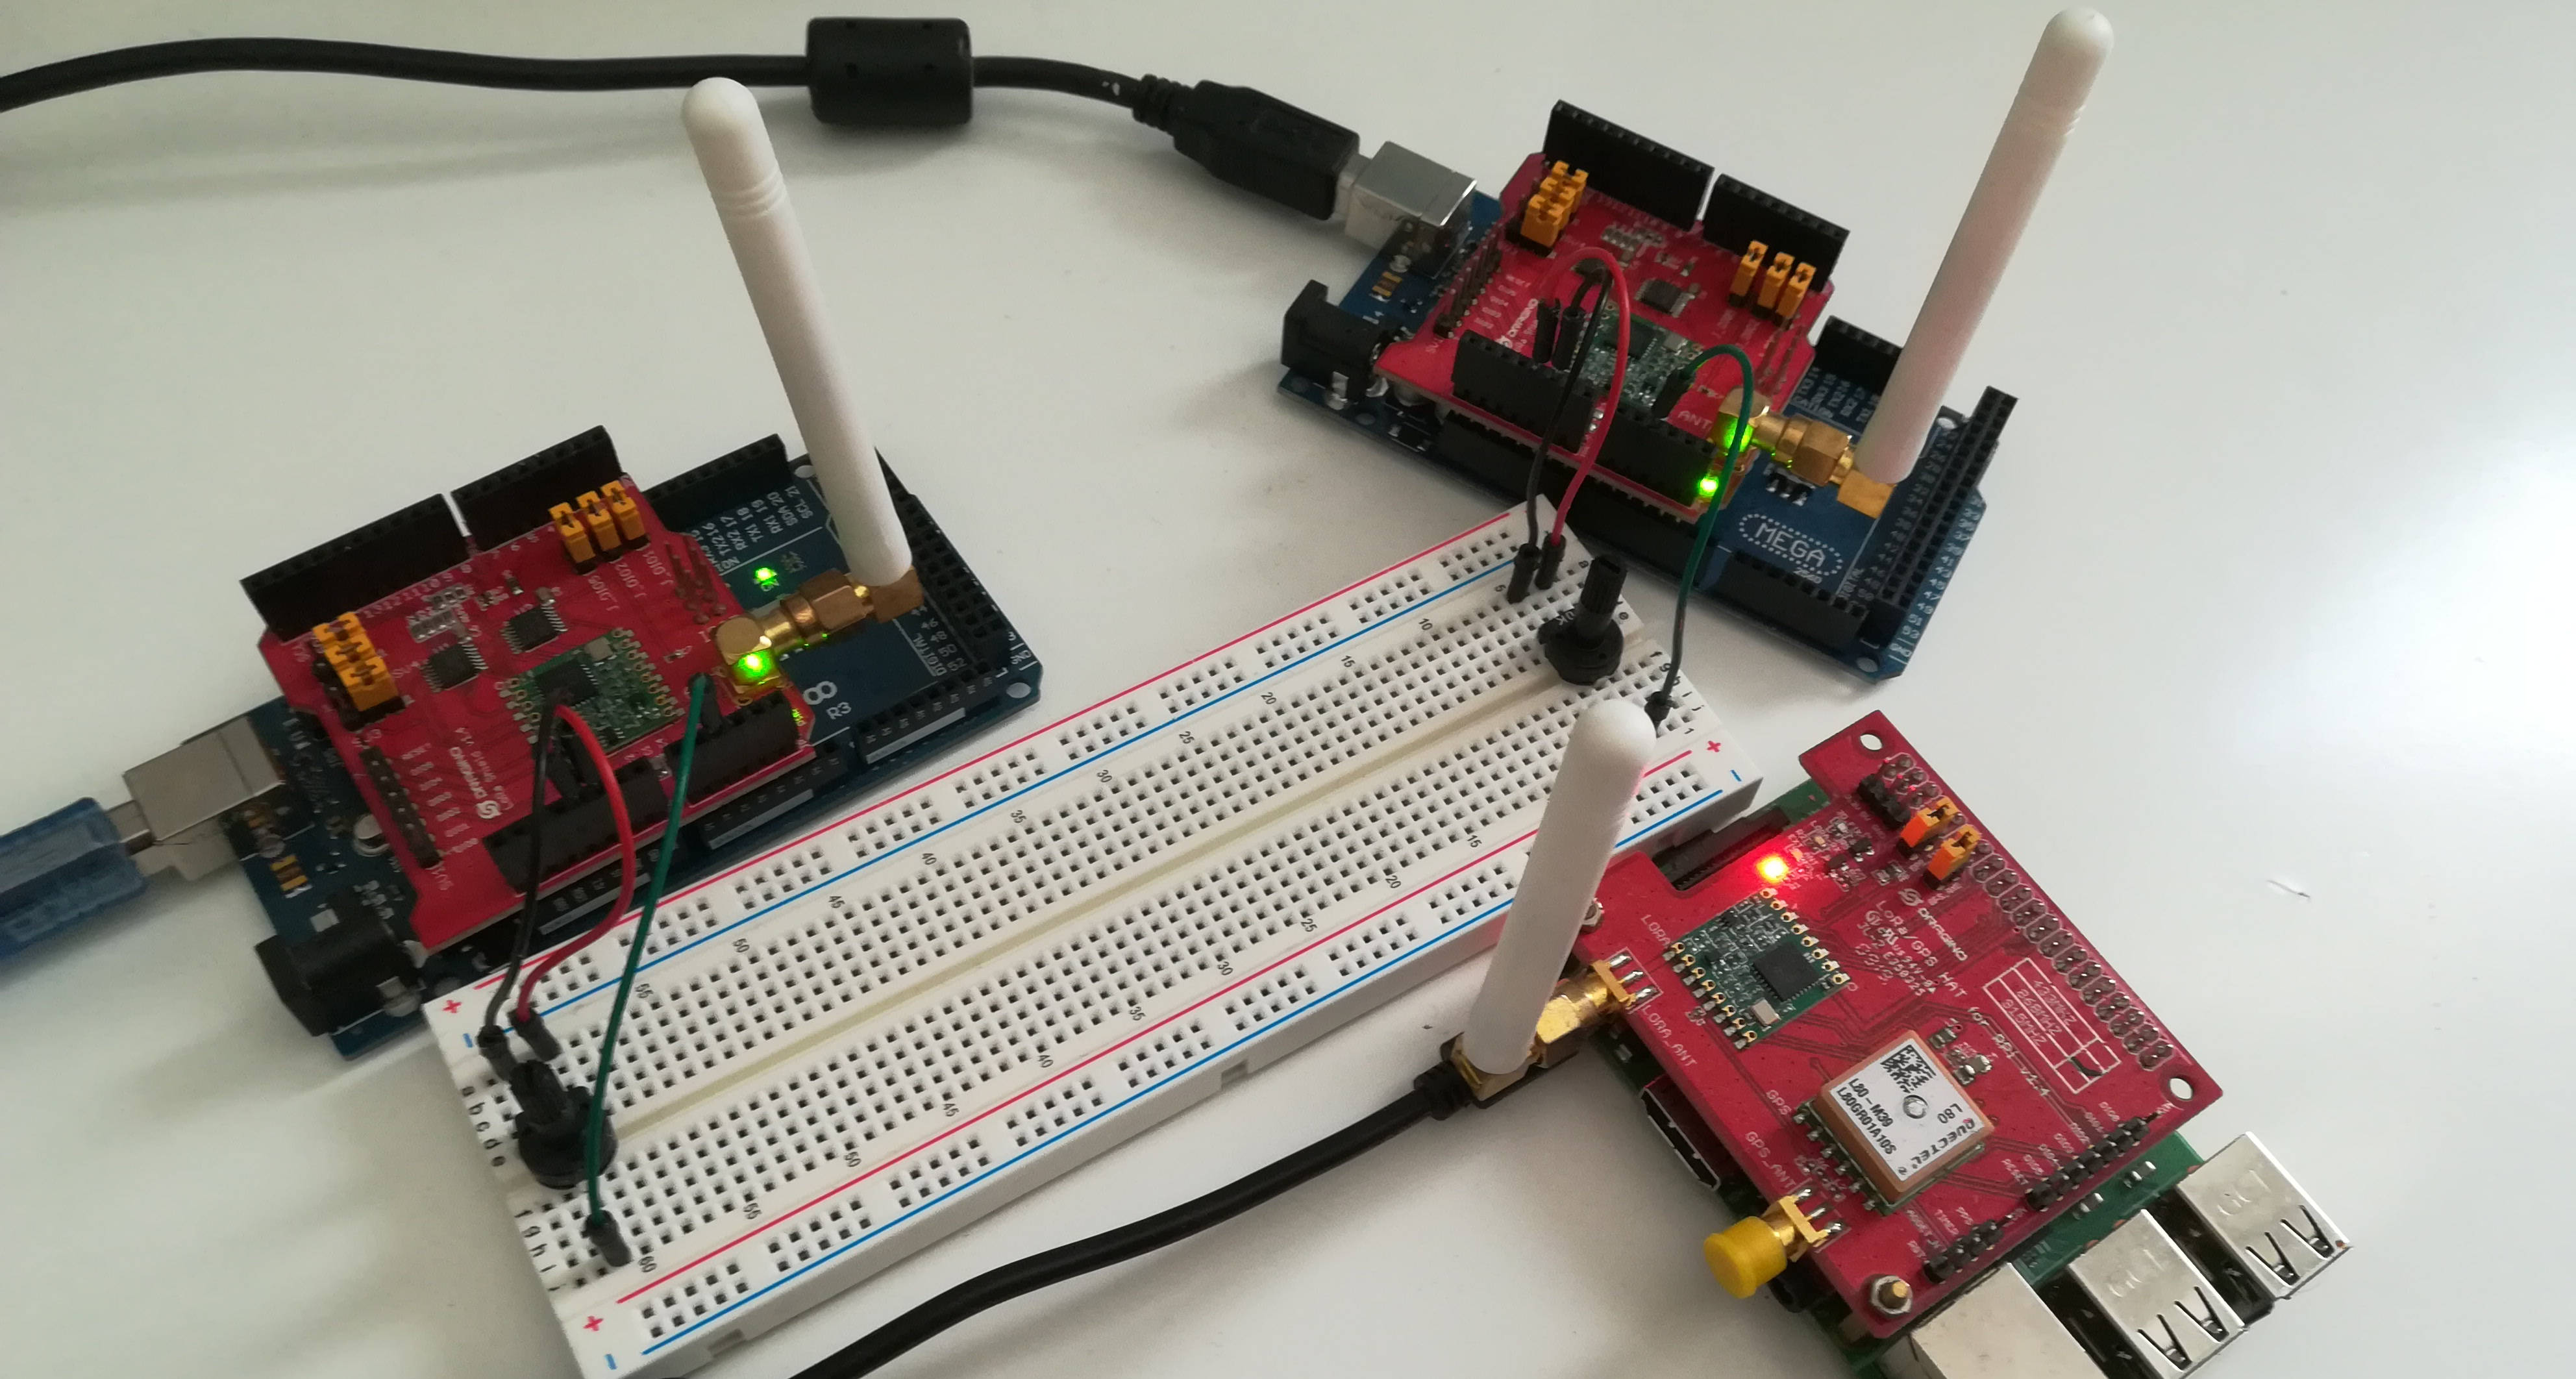
\includegraphics[width=.9\textwidth]{../pictures/2prototypes_1gateway.jpg}  
  \caption{Two prototypes transmitting through the gateway}
  \label{fig:2nodes_gateway}
\end{figure}

\subsection{Set up the gateway}
This process has been widely detailed in \ref{sssec:Gateway} subsection. The most important point on this stage is to ensure the systemd service is working properly and to retrieve the Gateway ID, which will be needed in the next stage.

\subsection{TTN Stack}
The first thing that must be done is to follow the three steps described in subsection \ref{sssec:TTN_Stack} ---Register a Gateway using its \enquote{Gateway ID}, Add an application and register a device for that application; this is the first step because the reader will need the security keys to two following stages:

\begin{itemize}
  \item Embebe these keys in Arduino sketch. This sketch will require the \enquote{Application Session Key}, \enquote{Network Session Key} and \enquote{Device Address}.
  \item Use them to create devices, and subscriptions in FIWARE. To create the device ---and also its corresponding entity and subscription when using the designed graphical interface shown in \ref{sssec:API_GUI} subsection--- the IoTagent will require the \enquote{Application ID}, \enquote{Application Access Key}, \enquote{Device ID}, \enquote{Application EUI} and again \enquote{Application Session Key}.
\end{itemize}

We must remember also it is so important to choose the CayenneLPP as the payload decoder. Once these keys are available in TTN platform, the process can continue.

\subsection{Customize the Arduino sketch for a specific device}
As indicated, this sketch will need the \enquote{Application Session Key}, the \enquote{Network Session Key} and \textbf{\enquote{Device Address}}, this latter is the most important key, because several nodes chan use the same \enquote{Application Session Key} and \enquote{Network Session Key}, but \enquote{Device Address} must be unique ---it is in fact also provided by TTN and the reader can check those are different for every node created in TTN platform. 

Of course, to be able to compile the sketch some dependencies must be satisfied, such as CayenneLPP ArduinoJson and lmic-arduino libraries. Moreover, the \textbf{linear potentiometer has been replaced for a rotary potentiometer}, again due to circumstances in the moment when the project is developed.

\begin{figure}[ht]
  \centering
  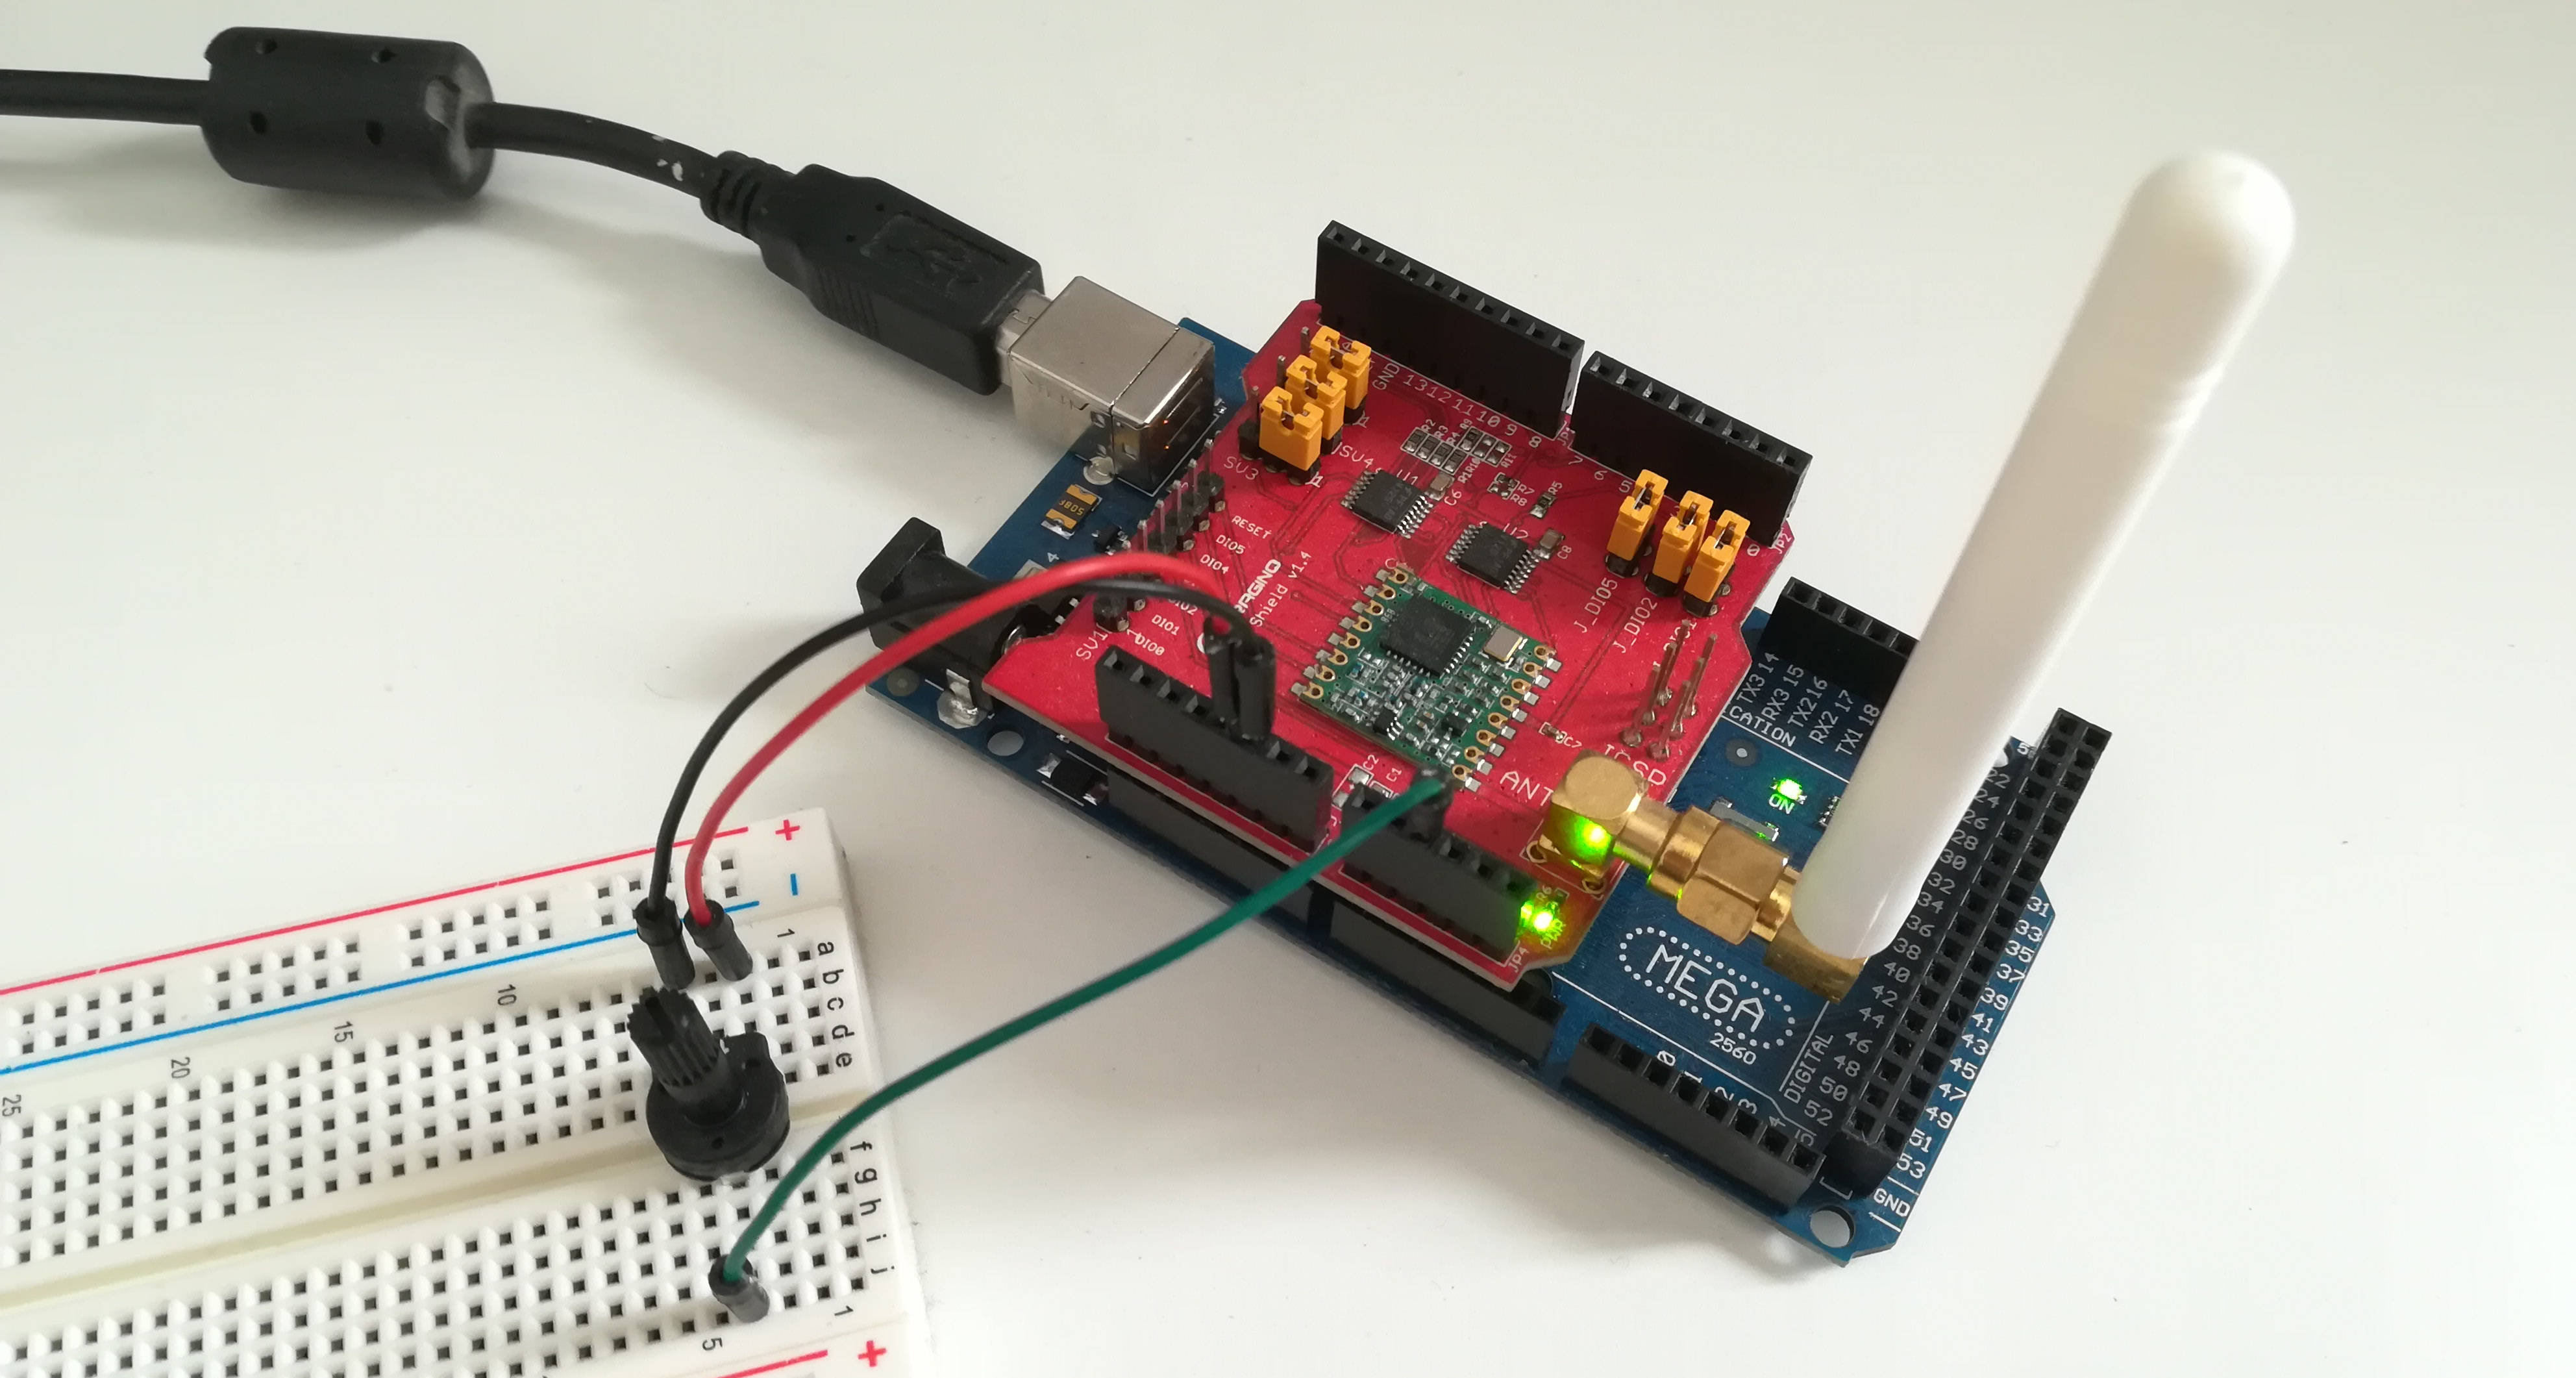
\includegraphics[width=.9\textwidth]{../pictures/prototype.jpg}
  \caption{Prototype broadcasting LoRa packets.}
  \label{fig:prototype}
\end{figure}

It's important to note that has been chosen the analog pin 2 for analog signal acquisition. Besides the reader can check the status of the device in serial monitor, however, the reader must also note that serial monitor is setup at 115200 bits per second.

\subsection{Deploy Docker containers}
Once the hardware has been properly setup, the next step is deploy locally all Docker containers, so as indicated in \ref{sssec:FIWARE} subsection, using \cmd{docker-compose} is possible to do this easily. 

This will deploy essentially the IoTagent-LoRaWAN, Orion CB, QuantumLeap and Grafana. The status of these containers can be checked by performing \cmd{docker ps -a}.

\subsection{Devices, entities and subscriptions}
When Docker containers are deployed, it should be possible to send HTTP requests to create a device (with its entity) and a subscription to notify QuantumLeap at any change for a particular entity. This process can be don by two different ways as indicated previously, 

\begin{itemize}
  \item Using developed graphical user interface (recommended, see \ref{sssec:API_GUI} subsection)
  \item Using \cmd{curl} or Postman to perform directly the HTTP requests
\end{itemize}

\subsection{Grafana}
Once any device (with an entity) and particularly its subscription are properly created, CrateDB should start journaling the context data, therefore next step is to add CrateDB as a data source in Grafana. 

So if the data source is properly added, it should be possible to create a new panel into a new dashboard, setting up the proper query for that panel, Grafana should start to plot the context data. (see \ref{sssec:Grafana} subsection for further details)

Finally the system it would be completely deployed and journaling the context data, as it can be seen in figure \ref{fig:final_panel}.

\clearpage{\pagestyle{empty}\cleardoublepage}\pagestyle{plain}  % Forces the next section to start in an odd page.
\section{Conclusions}
Finally there are a few considerations that could be done, 

\begin{itemize}
  \item A rotary potentiometer does work well enough as a proof of concept, but would have been more appropriate to have the expected linear potentiometer to try its sensibility, which is a good point in order to measure such little variations as produced in the stem diameter in a tree.
  \item The fact that the Raspberry Pi HAT uses a single channel chip (SX1276) has two important implications:
    \begin{itemize}
      \item In a first place, as indicated in its corresponding section, these kind of gateways are LoRaWAN compatible but not compliant. So it would be desirable to replace this HAT by another one, or simple to acquire a proper gateway for a production environment.
      \item Secondly, Nodes cannot comunicate simultaneously with the gateway because it is listening only one channel, so this is causing a time gap in data acquisition as it can be seen in the picture \ref{fig:times_gap}
      \begin{figure}[ht]
        \centering
        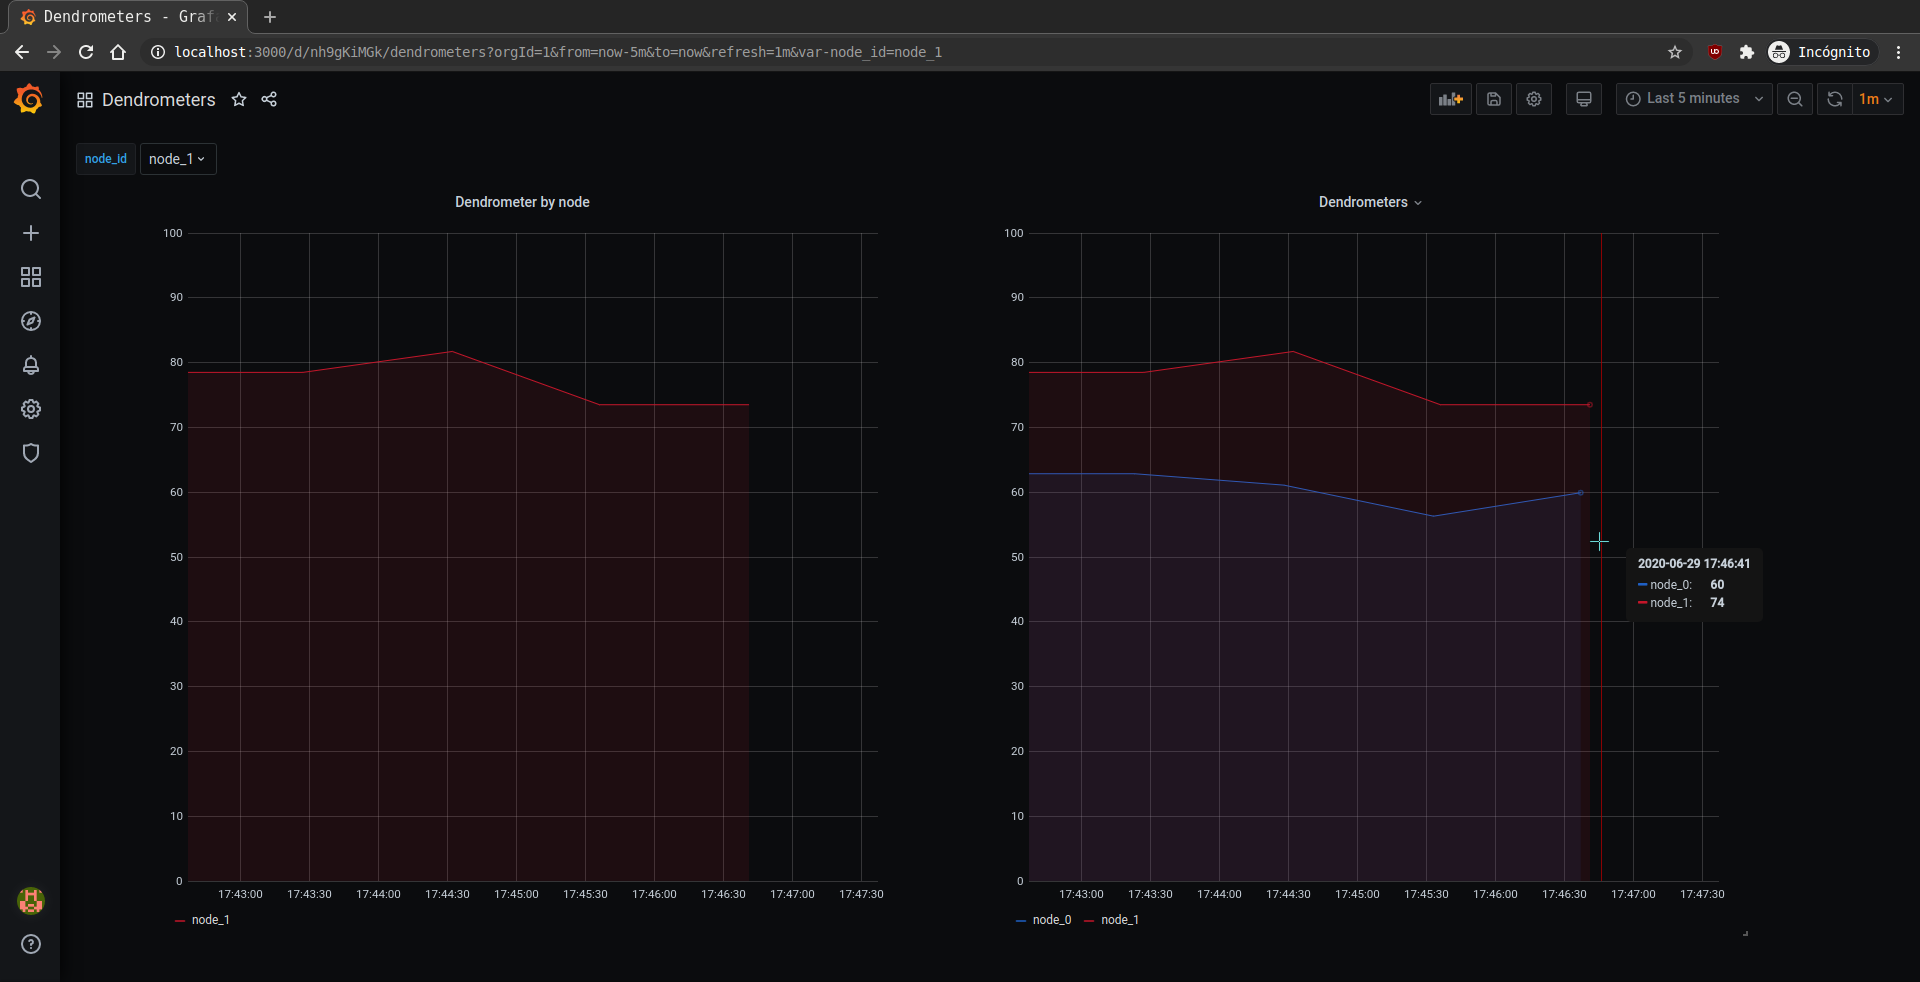
\includegraphics[width=.9\textwidth]{../pictures/Grafana_times_gap.png}
        \caption{Little gap between times caused by the single channel chip.}
        \label{fig:times_gap}
      \end{figure}
    \end{itemize}
    \item End-nodes are being activated using ABP method, this method could not be as effective as OTAA method in the case that downlinks packets were transmitted, this is why due to some security implications frame counters must be reset for ABP devices every time they are shutdown for any circumstance; in particular when downlinks are transmitted, could be necessary to reset the frame counter in the devices, so in this situation would be interesting to consider swap to OTAA method. In fact, TTN offers the possibility to reset the frame counter in TTN console but this could be removed in a future.
    \item Maybe the developed GUI could have handle also the context data plots, however this project couldn't have covered in anyway this development with the available time, so this is not considered as part of the project because Grafana is complete enough to this task for now and perhaps for ever due to it is extremely powerful handling databases.
    \item For a production environment it seems clear that arduino devices should be encapsulated and the sensor (potentiometer) part must be improved; however this is not hard because of the wide offer for cases and power supply systems, this would lead a very compact device which could be also improved adding more sensor due to versatility of CayenneLPP encoding standard which allows to send multiple measurements of different sensors. 
    \item Finally this project is a good candidate to replace expensive commercial and proprietary systems; so it likely keeps developing, depending on the needs of the researchers.
\end{itemize}

\clearpage{\pagestyle{empty}\cleardoublepage}\pagestyle{myfancy} % Forces the next section to start in an odd page.
\phantomsection\addcontentsline{toc}{section}{References}
\printbibliography
\end{document}
